\chapter{Substructure Discovery in Tandem Mass Spectometry Data}
\label{c:background}

\section{Introduction}

Unlike the previous chapters where the mass spectrometry data to be analysed is produced through measurements from a single MS instrument, in this chapter, the application of probabilistic methods to the discovery of patterns in tandem mass spectrometry (MS2) fragmentation data is introduced. As discussed in Section~\ref{sub:identification-background}, analysis of MS metabolomics data is challenging since many molecules cannot be identified from their mass alone (e.g. isobaric molecules, and isomers) \cite{VanderHooft2013, Kind2006}. Separation by liquid chromatography prior to mass spectrometry can add discriminatory information but does not solve the problem as isomers can exhibit similar chromatographic behavior, and chromatographic retention time is unpredictable. From a tandem-MS set-up, fragmentation spectra can be obtained that are characteristic of the structural composition of the precursor ions that generate them, and through the matching against public spectra library, these fragmentation spectra can be used to annotate the identities of the metabolites present in the sample. However, spectral identification itself cannot completely address the identification problem due to the limited number of reference spectra present in databases (e.g. MassBank, HMDB) that a query spectra can be matched against. 

Following the assumption that each observed spectrum is comprised of one or more such substructures, an unsupervised analysis workflow is proposed that reduces the large number of fragmentation spectra to sets of co-occurring molecular fragments and neutral losses. This is accomplished through the application of the Latent Dirichlet Allocation (LDA) model to spectral fragmentation data. The proposed workflow, called 'MS2LDA', converts fragmentation spectra into 'documents' of fragment and neutral loss 'word' features and produces as output the sets of topics shared by documents. In the context of fragmentation data, we define a \textit{Mass2Motif} to be a topic that potentially corresponds to a biochemically-relevant molecular substructure shared by many metabolites. 

The results of MS2LDA analysis allows us to immediately explore the biochemistry present in the sample via the relative abundance of a small number of different molecular substructures that, based on our analysis, are often straightforward to annotate. The presence of shared substructures allows us to group metabolites in a meaningful way even if they do not share a large degree of overall spectral similarity. If many molecules in such a group share a pattern of differential expression, we can hypothesise the cause of the change in abundance without having to identify all of the metabolites and map them to a metabolic pathway. Presence of substructures can also be used to provide putative annotations or functional classifications for metabolites that are otherwise unidentifiable. Changes to the expression levels of substructures can also be examined from the resulting output of MS2LDA. Finally, from the results of performing independent multiple MS2LDA structural annotations on different biological samples, an extension to the standard LDA model is introduced that allows the sharing of topics across multiple runs. The extended LDA model allows the presence of topics to be jointly inferred across multiple runs at once, eliminating the need for the tedious manual matching of topics that occur across runs.

\section{Related Work}

Recurring patterns of fragments (product ions) and neutral losses that are present in fragmentation spectra can be explained by the presence of common biological substructures (e.g. a hexose unit, or a CO loss) in metabolites. The representation of small molecules as combinations of building blocks has previously been used for the annotation of a small number of molecules in direct infusion-MS with fragmentation \cite{Sweeney2014} and for metabolite classification in GC-MS \cite{Scott1994, Hummel2010}. CSI:FingerID ranks candidate molecules based on the presence and absence of various predefined structural features, including substructures \cite{Duhrkop2015}. These studies reveal the potential of substructure-based approaches in MS but require structurally known training data, which is costly to produce and often platform-specific. 

Tools exist that operate on the entire fragmentation spectra. For example, “Molecular Networking” clusters MS1 peaks by their MS2 spectral similarity such that one identifiable metabolite in a cluster facilitates structural annotation of its neighbors \cite{yang2013molecular, van2016urinary}.  However, spectral features causing the clustering must be extracted manually and only MS2 spectra with high overall spectral similarity are grouped. Another package, MS2Analyzer \cite{ma2014ms2analyzer} mines MS2 spectra for specific features defined by the user (i.e., mass fragments and neutral losses). Some will be common to many experiments (e.g. CO or H2O losses), but sample-specific features are easily overlooked. Whilst Molecular Networking requires no user intervention it may fail to group molecules that share small substructures, whilst MS2Analyzer can find all molecules that share a particular set of features provided they are user-specified. 

The approach in this chapter, MS2LDA, is based on Latent Dirichlet Allocation (described in Section~\ref{background-lda}) and retain the benefits of entire spectra-oriented tools whilst losing the shortfalls --- it can find relevant substructures based on the co-occurrence of mass fragments and neutral losses, and group the molecules accordingly. LDA was previously adapted to other types of high throughput data (genomics \cite{chen2010probabilistic}, metagenomics \cite{zhang2015exploiting}, and transcriptomics \cite{rogers2005latent}) but never before to exploit the parallels between MS2 fragmentation data and text.

\section{A Workflow for Substructure Discoveries and Annotations}

The key insight to the MS2LDA workflow lies in the parallel between text and MS fragmentation data (Figure~\ref{fig:text2frags}). As a text analysis pipeline relying on LDA decomposes documents into topics based on frequently co-occurring words, so MS2LDA decomposes fragmentation spectra into their constituent building blocks of frequently co-occurring fragments and neutral losses (referred to as ‘Mass2Motifs’). Crucially, MS2LDA achieves this with an unsupervised manner, using all of the fragmentation spectra generated by data-dependent mass fragmentation analysis (DDA) to learn the decomposition of the fragmentation spectra into potential chemically-relevant substructures. 

\begin{figure}[!htbp]
\centering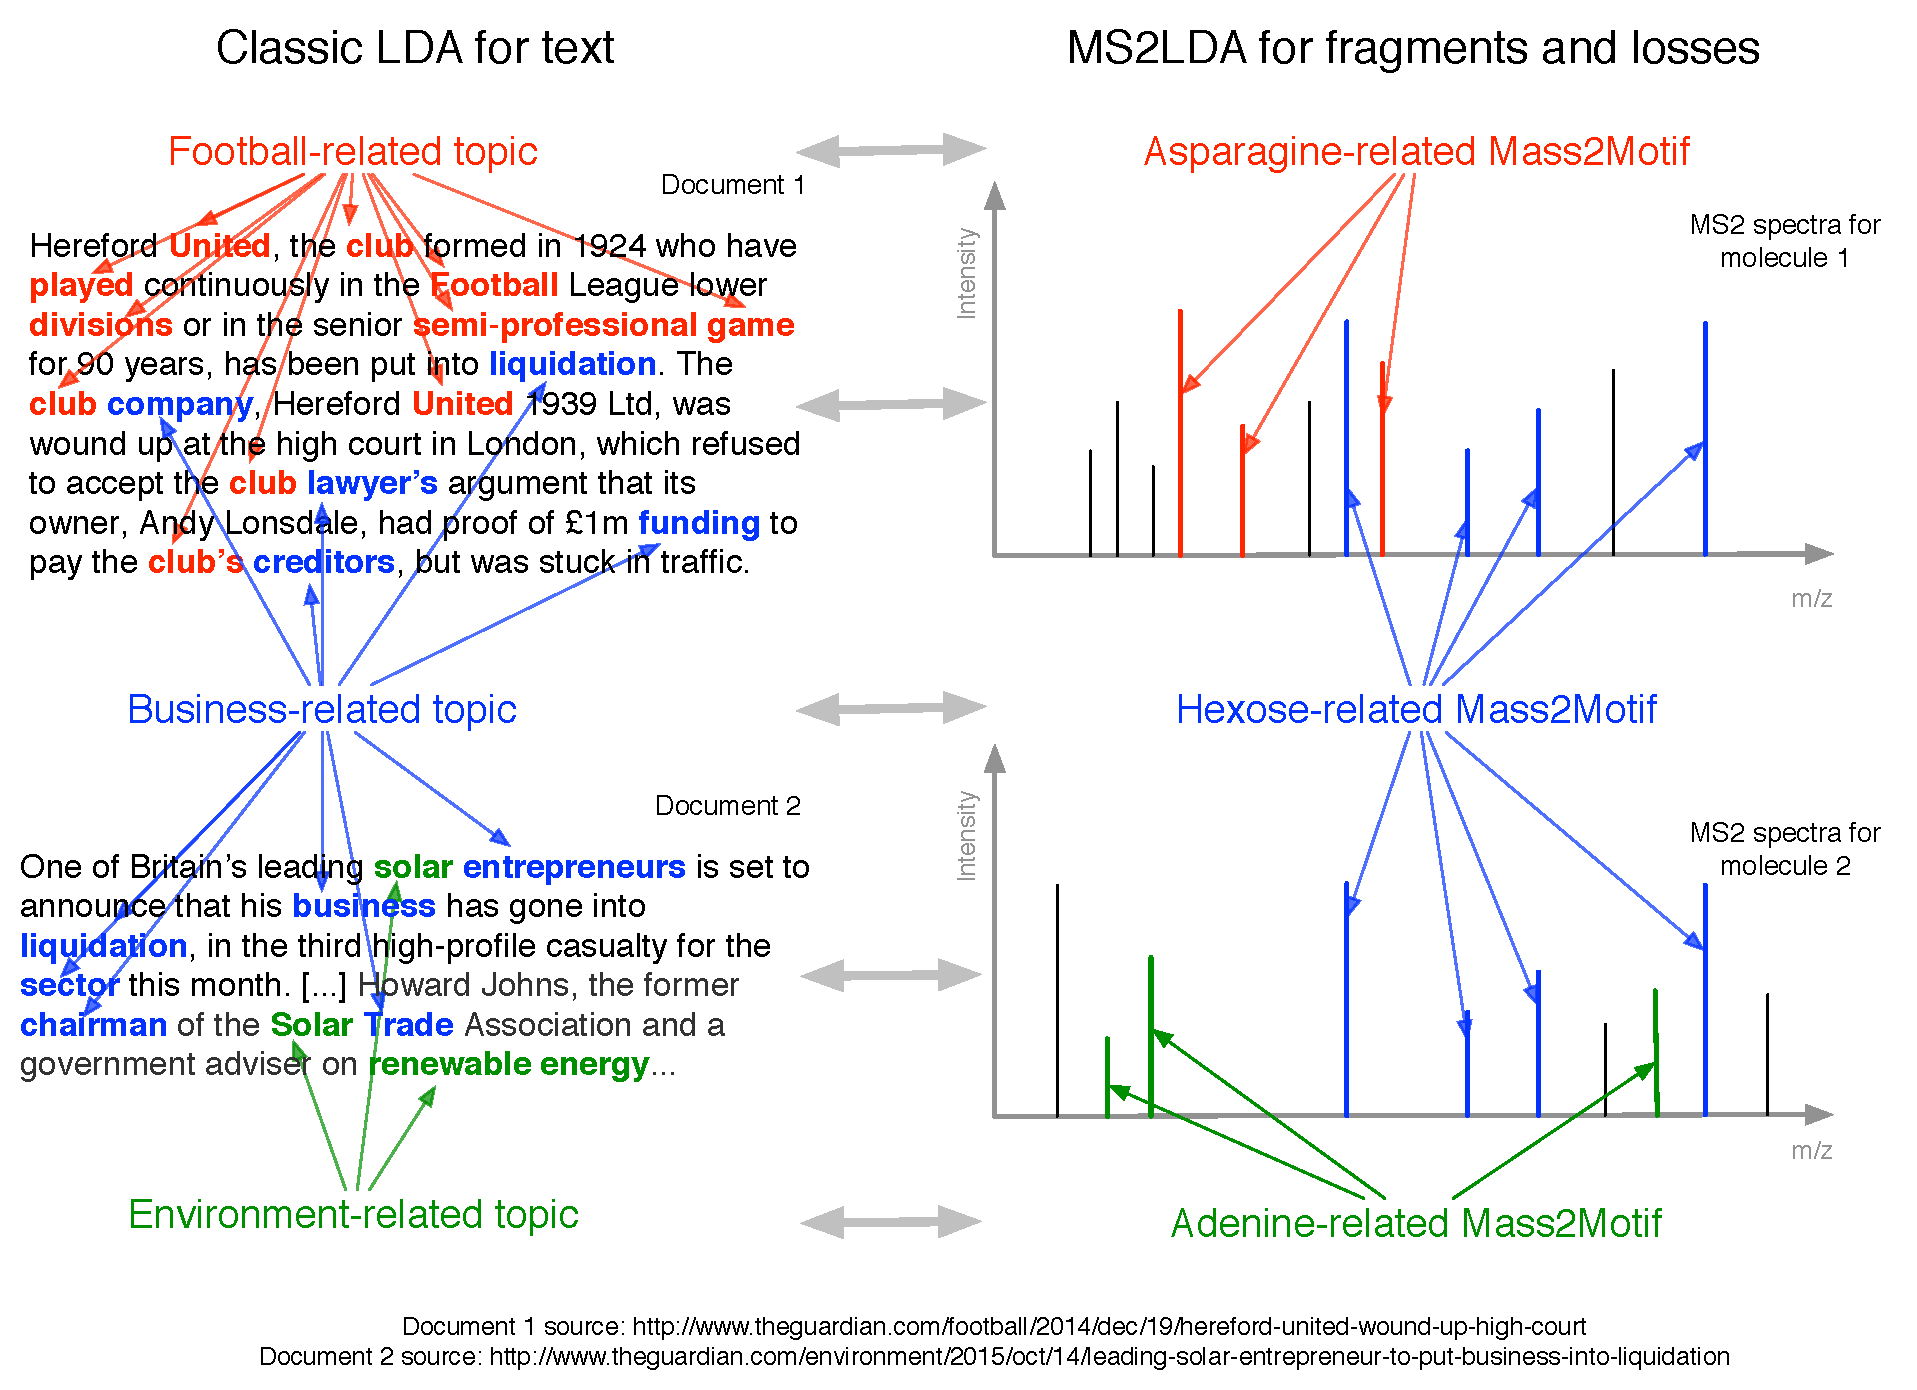
\includegraphics[width=0.6\linewidth]{07-lda/figures/text2frags.pdf}
\centering\caption{Figure 1: Analogy between LDA for text-mining and MS2LDA. Traditional LDA extract topics that can be interpreted as ‘football related’, ‘business-related’ and ‘environment related’, with each document a combination of different topics. Similarly, MS2LDA extracts different sets of co-occuring mass fragments or losses (Mass2Motifs) from the fragmentation spectra that can be interpreted as ‘Asparagine-related’, ‘Hexose-related’ and ‘Adenine-related’. Each fragmentation spectra comprise of one or more Mass2Motifs.\label{fig:text2frags}}
\end{figure}

The MS2LDA workflow consists of two stages: i) the data conversion stage, which prepares the acquired fragmentation data into suitable input format for the workflow, followed by ii) the Mass2Motif discovery stage, which performs topic modelling via LDA to discover mass fragmental patterns, assigns potential candidate elemental formulae to MS1 and MS2 peaks, and visualises the Mass2Motifs in an interactive environment. The complete workflow is illustrated in Figure~\ref{fig:m2lda-workflow} and described in more details in the following Section~\ref{sub:data-conversion} and \ref{sub:topic-discovery}.

\begin{figure}[!htbp]
\centering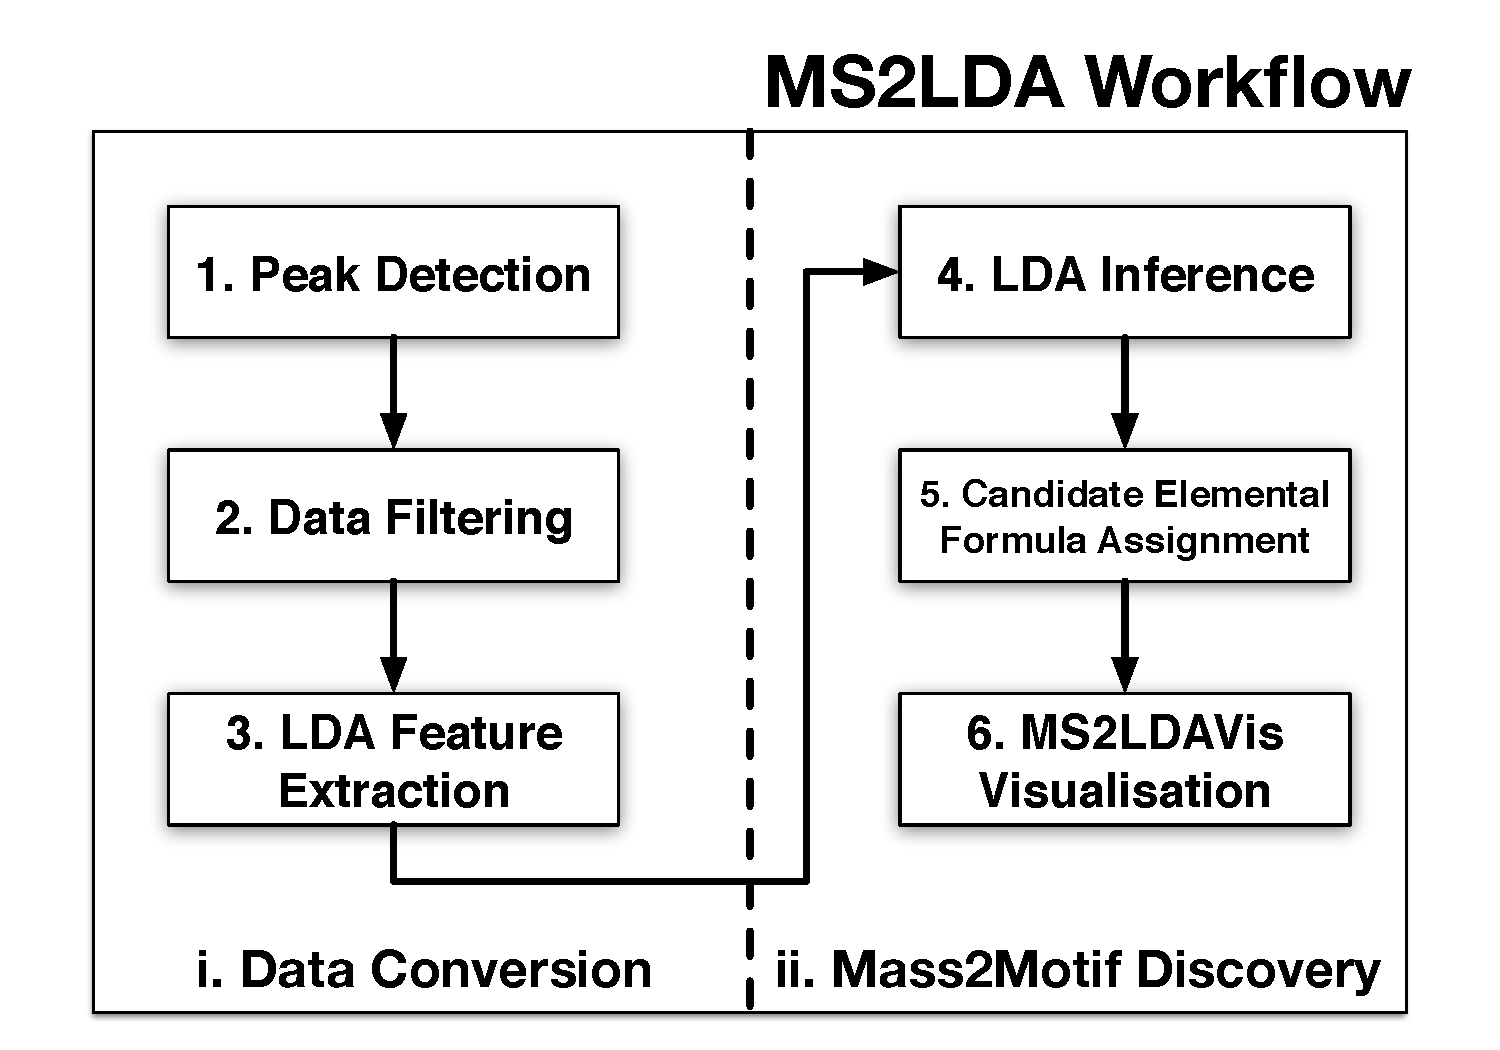
\includegraphics[width=0.6\linewidth]{07-lda/figures/ms2lda.pdf}
\centering\caption{Schematic overview of the MS2LDA workflow..\label{fig:m2lda-workflow}}
\end{figure}

\subsection{Data Conversion\label{sub:data-conversion}}

\subsubsection{Peak Detection \& Data Filtering}

Data conversion is an essential part of the MS2LDA workflow, since the acquired fragmentation data cannot readily be used for the purpose of mass fragmental pattern searching. As input, the workflow accepts the combination of a single full-scan file for the MS1 peaks and a separate fragmentation file for the MS2 peaks. The data conversion process starts with the detection of MS1 peak in the input .mzXML file obtained from full-scan mode spectra using the CentWave algorithm from the XCMS library \cite{Smith2006}. This constitutes information on the MS1-level. Fragmentation data, in the form of .mzML file obtained from tandem MS mode, are processed using an R script based on the RMassBank package \cite{Stravs2013}. The script performs a greedy search for the most intense unique MS2 spectrum that can be linked to an MS1 LC-MS peak within a specified retention time (RT) window. A filtering step based on RT and intensity is applied to remove noisy peaks, as well as the washing part, equilibration part, and the start of the chromatogram prior to the injection peak. Any MS1 peak not having paired MS2 peaks is subsequently discarded for further processing. The aim of the filtering step is to exclude identical fragmentation spectra produced by low-intensity MS1 peaks that were fragmented multiple times, which could potentially forming a topic on their own. 

\subsubsection{LDA Feature Extraction}

The next step in the data conversion stage is the transformation of the spectral data into a suitable input format, which is a matrix consisting of the MS1 peaks (columns) and their correspondent MS2 word features (rows) (see Figure~\ref{fig:m2lda-matrix}). In LDA applied to the text domain, this corresponds to the matrix of counts of word occurrences in documents. Similarly, each MS1 peak can now be seen as a ‘document’ while the linked MS2 spectrum associated to each MS1 peak produce the ‘word’ features in a document. Following the bag-of-words assumption, LDA does not take into account word orders, but instead consider the number of times a word occurs in a document. 

\begin{figure}[!htbp]
\centering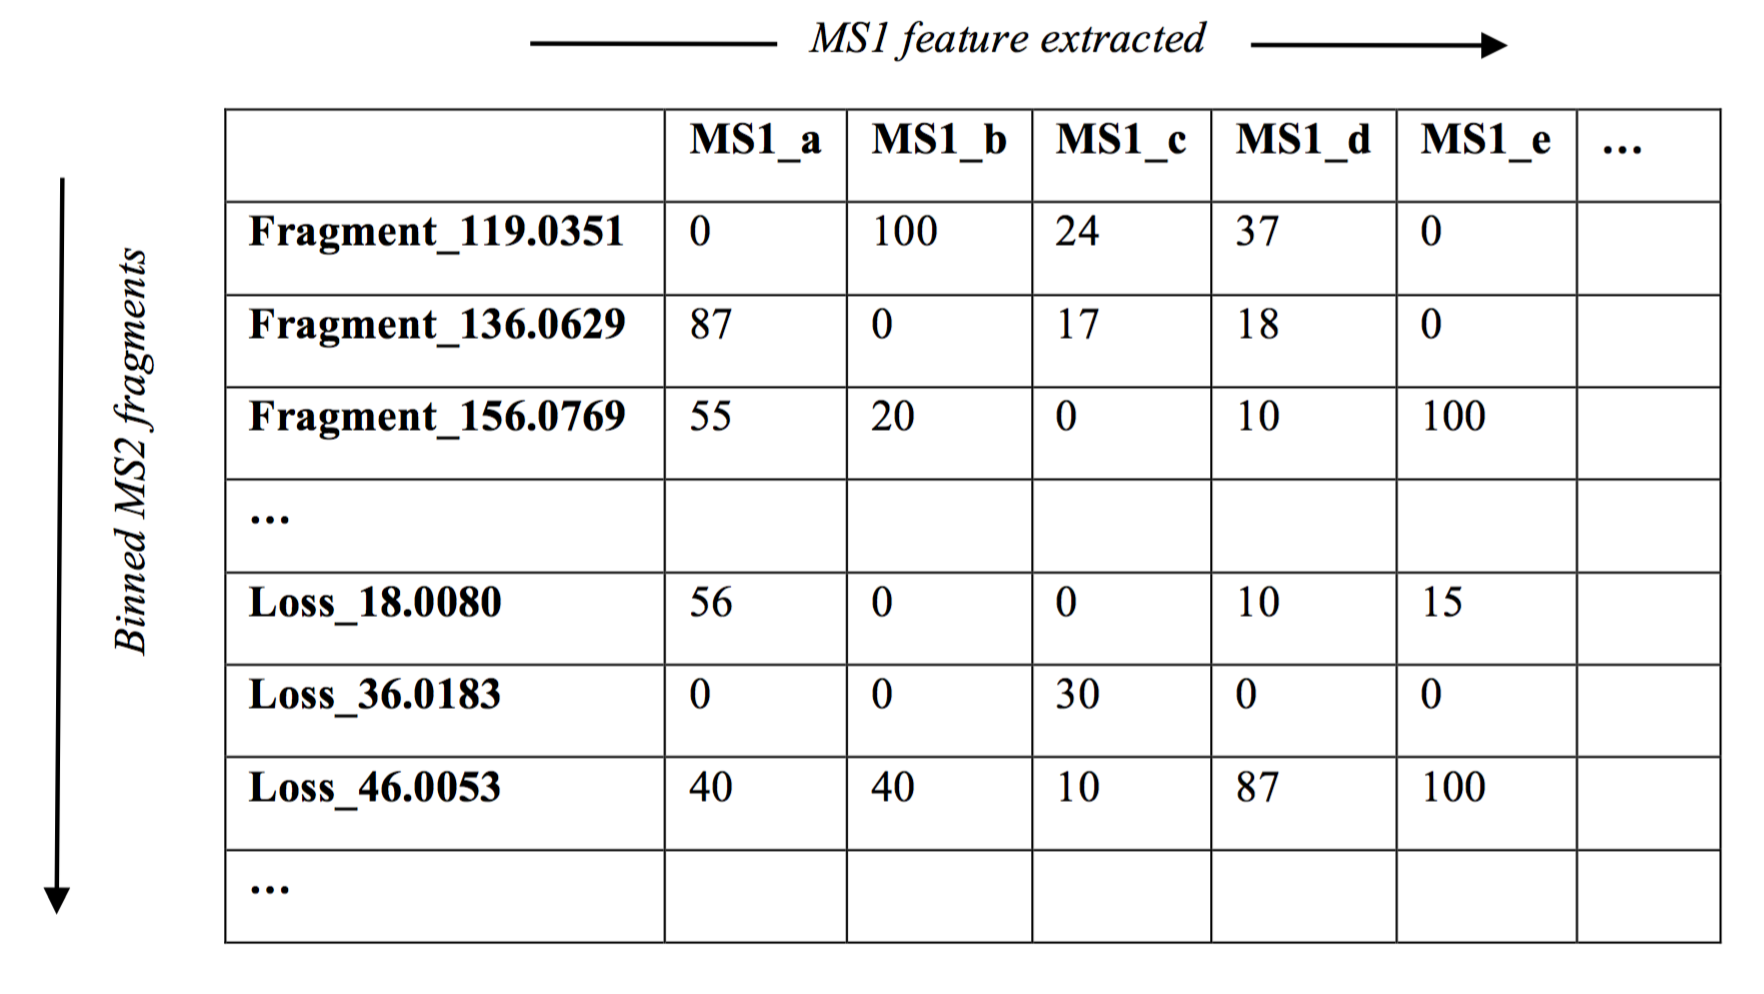
\includegraphics[width=0.8\linewidth]{07-lda/figures/matrix.png}
\centering\caption{The data-frame extracted from fragmentation data: a matrix of XCMS-picked MS1 peaks (columns) and binned mass fragment (and neutral loss) features with normalized (0 – 100 scale) intensities.\label{fig:m2lda-matrix}}
\end{figure}

For each MS1 peak, two types of word features can be extracted from the MS2 fragmentation spectrum:
\begin{itemize}
\item \textbf{Fragment features}, which are the discretized mass values of the MS2 peaks. A greedy binning process is used to group MS2 peaks within a certain user-defined m/z window from the next unprocessed MS2 peak. This way, MS2 peaks with close-enough m/z values but observed in different precursor MS1 peaks are linked and placed into the same discrete bin – each bin corresponds to a fragment feature. The input for inference in textual LDA is the count of occurrences of words in each document; in MS2LDA, the intensity values of MS2 peaks can be considered to be proxies for word counts. These intensity values are normalized by dividing to the largest intensity value in the fragmentation spectrum and discretized on a scale of 0 to 100 (integers). 
\item \textbf{Loss features}, which is the discretized mass values of the neutral losses. Neutral losses are the mass differences between a precursor MS1 peak and each of its MS2 peaks in the spectrum. To produce the loss features, we find the m/z difference between each fragment MS2 peak to its parent MS1 peak. Similar to fragment features, the normalized intensity values of the neutral losses, represented by the intensities of their resulting mass fragments, are used as proxies for the loss counts.
\end{itemize}

\subsection{Mass2Motif Discovery\label{sub:topic-discovery}}

\subsubsection{LDA Inference}

After the data conversion step, the resulting matrix has MS2 features (fragments and losses) as rows and columns corresponding to the MS1 peaks. The values in the matrix are the MS2 feature intensities which are subsequently turned into integer counts by normalising and rounding such that the most intense feature for each MS1 peak has value 100. LDA is applied to perform the unsupervised discovery of Mass2Motifs in the data. In the context of fragmentation data, the standard LDA model --- as applied to substructure discovery --- is described next. The observation on the $n$-th fragment or loss feature in the $d$-th fragmentation spectra ($w_{dn}$) is conditioned on the assignment of feature $w_{dn}$ to the $k$-th Mass2Motif multinomial distribution. This assignment is denoted by the indicator variable $z_{dn}$, so $z_{dn}=k$ if feature $w_{dn}$ is assigned to a $k$-th Mass2Motif. The $k$-th multinomial distribution that a feature is assigned to is characterised by the parameter vector $\boldsymbol{\phi}_{z_{dn}}$, with $\boldsymbol{\phi}_{z_{dn}}$ drawn from a prior Dirichlet distribution with a symmetric parameter $\beta$. 
\begin{align}
w_{dn} \vert \boldsymbol{\phi}_{z_{dn}} &\sim Multinomial(\boldsymbol{\phi}_{z_{dn}}) \\
\boldsymbol{\phi}_{k} \vert \beta &\sim Dirichlet(\beta)
\end{align}
The probability of seeing certain Mass2Motifs for each $d$-th fragmentation spectra is drawn from a multinomial distribution with a parameter vector $\boldsymbol{\theta}_{d}$. This parameter vector $\boldsymbol{\theta}_{d}$ is in turn drawn from a prior Dirichlet distribution having a symmetric parameter $\alpha$. 
\begin{align}
z_{dn} \vert \boldsymbol{\theta}_{d} &\sim Multinomial(\boldsymbol{\theta}_{d}) \\
\boldsymbol{\theta}_{d} \vert \alpha &\sim Dirichlet(\alpha)
\end{align}
A collapsed Gibbs sampling scheme is implemented in Python for inference (details in Section~\ref{background-lda}). The output from inference is a set of Mass2Motifs and assignments of Mass2Motifs to each MS1 peak. 

\subsubsection{Candidate Elemental Formula Assignment}

To aid data interpretation, putative elemental formulae can be displayed alongside the plots of fragmentation spectra that can be explained by a certain Mass2Motif (top-right panel, Figure~\ref{fig:m2ldavis-main}). MS2LDA provides two optional methods to assign candidate elemental formulae to the mass fragments, neutral losses, and precursor ions.  The first is achieved by integrating SIRIUS \cite{Bocker2009} into our workflow. SIRIUS assigns elemental formula by posing it as an integer decomposition problem and solving it through a dynamic programming approach ('Round Robin') \cite{Bocker2007}. SIRIUS is freely-available and, as it is written in Java, can in theory be run platform-independently on any Windows, Unix and Mac environment (in practice, library dependencies have to be satisfied before SIRIUS can be run on the target computer). Integration of SIRIUS into our workflow is achieved by wrapping calls to the Java package of SIRIUS through a separate sub-process, passing it a temporary MGF file that corresponds to each fragmentation spectrum. SIRIUS assigns elemental formulae to each combination of MS1 and MS2 peaks independently, which may lead to mass fragments of similar m/z value being assigned an elemental formula in some spectra, but not in all.

As an alternative strategy for annotation, MS2LDA also provides a pure Python implementation of an elemental formula assigner (called 'EF-Assigner') based on the Round Robin algorithm that also lies at the heart of SIRIUS. Once the initial assignment of potential candidate formulae to mass fragments, neutral losses and also precursor ion masses has been performed, the list of candidate formulae is further filtered using our implementation of the 7-golden rules, a set of heuristic rules introduced in \cite{Kind2007}. This filtering step is used to remove chemically-unlikely elemental formula compositions from the candidate list. Advantages of the EF-Assigner module are its easy integration with the rest of the workflow (it is also written in Python) and it assigns elemental formulae to the binned fragments and losses in the matrix instead of to individual spectra. However, unlike SIRIUS that uses the complete information of the precursor ion and fragments peaks in a spectrum for annotation, EF-Assigner assigns the elemental formulae for the MS1 peaks, mass fragments and neutral losses independently. 

\subsubsection{MS2LDAVis Visualisation\label{sub:ms2lda-visualisation}}

Given its hypothesis-generating nature, the analysis of Mass2Motifs to characterise and examine their correspondence to actual biochemical substructures is an iterative and exploratory process. In the MS2LDA workflow, this is made possible through the MS2LDAVis module --- an interactive web-based visualisation build upon the combination of the Javascript and the D3 library (http://d3js.org). MS2LDAVis is extended from the Python port of the topic modelling visualisation interface LDAVis \cite{Sievert2014} used in the text domain, but our adaptation in the form of MS2LDAVis introduces fragmentation-specific views.

\begin{figure}[!htbp]
\centering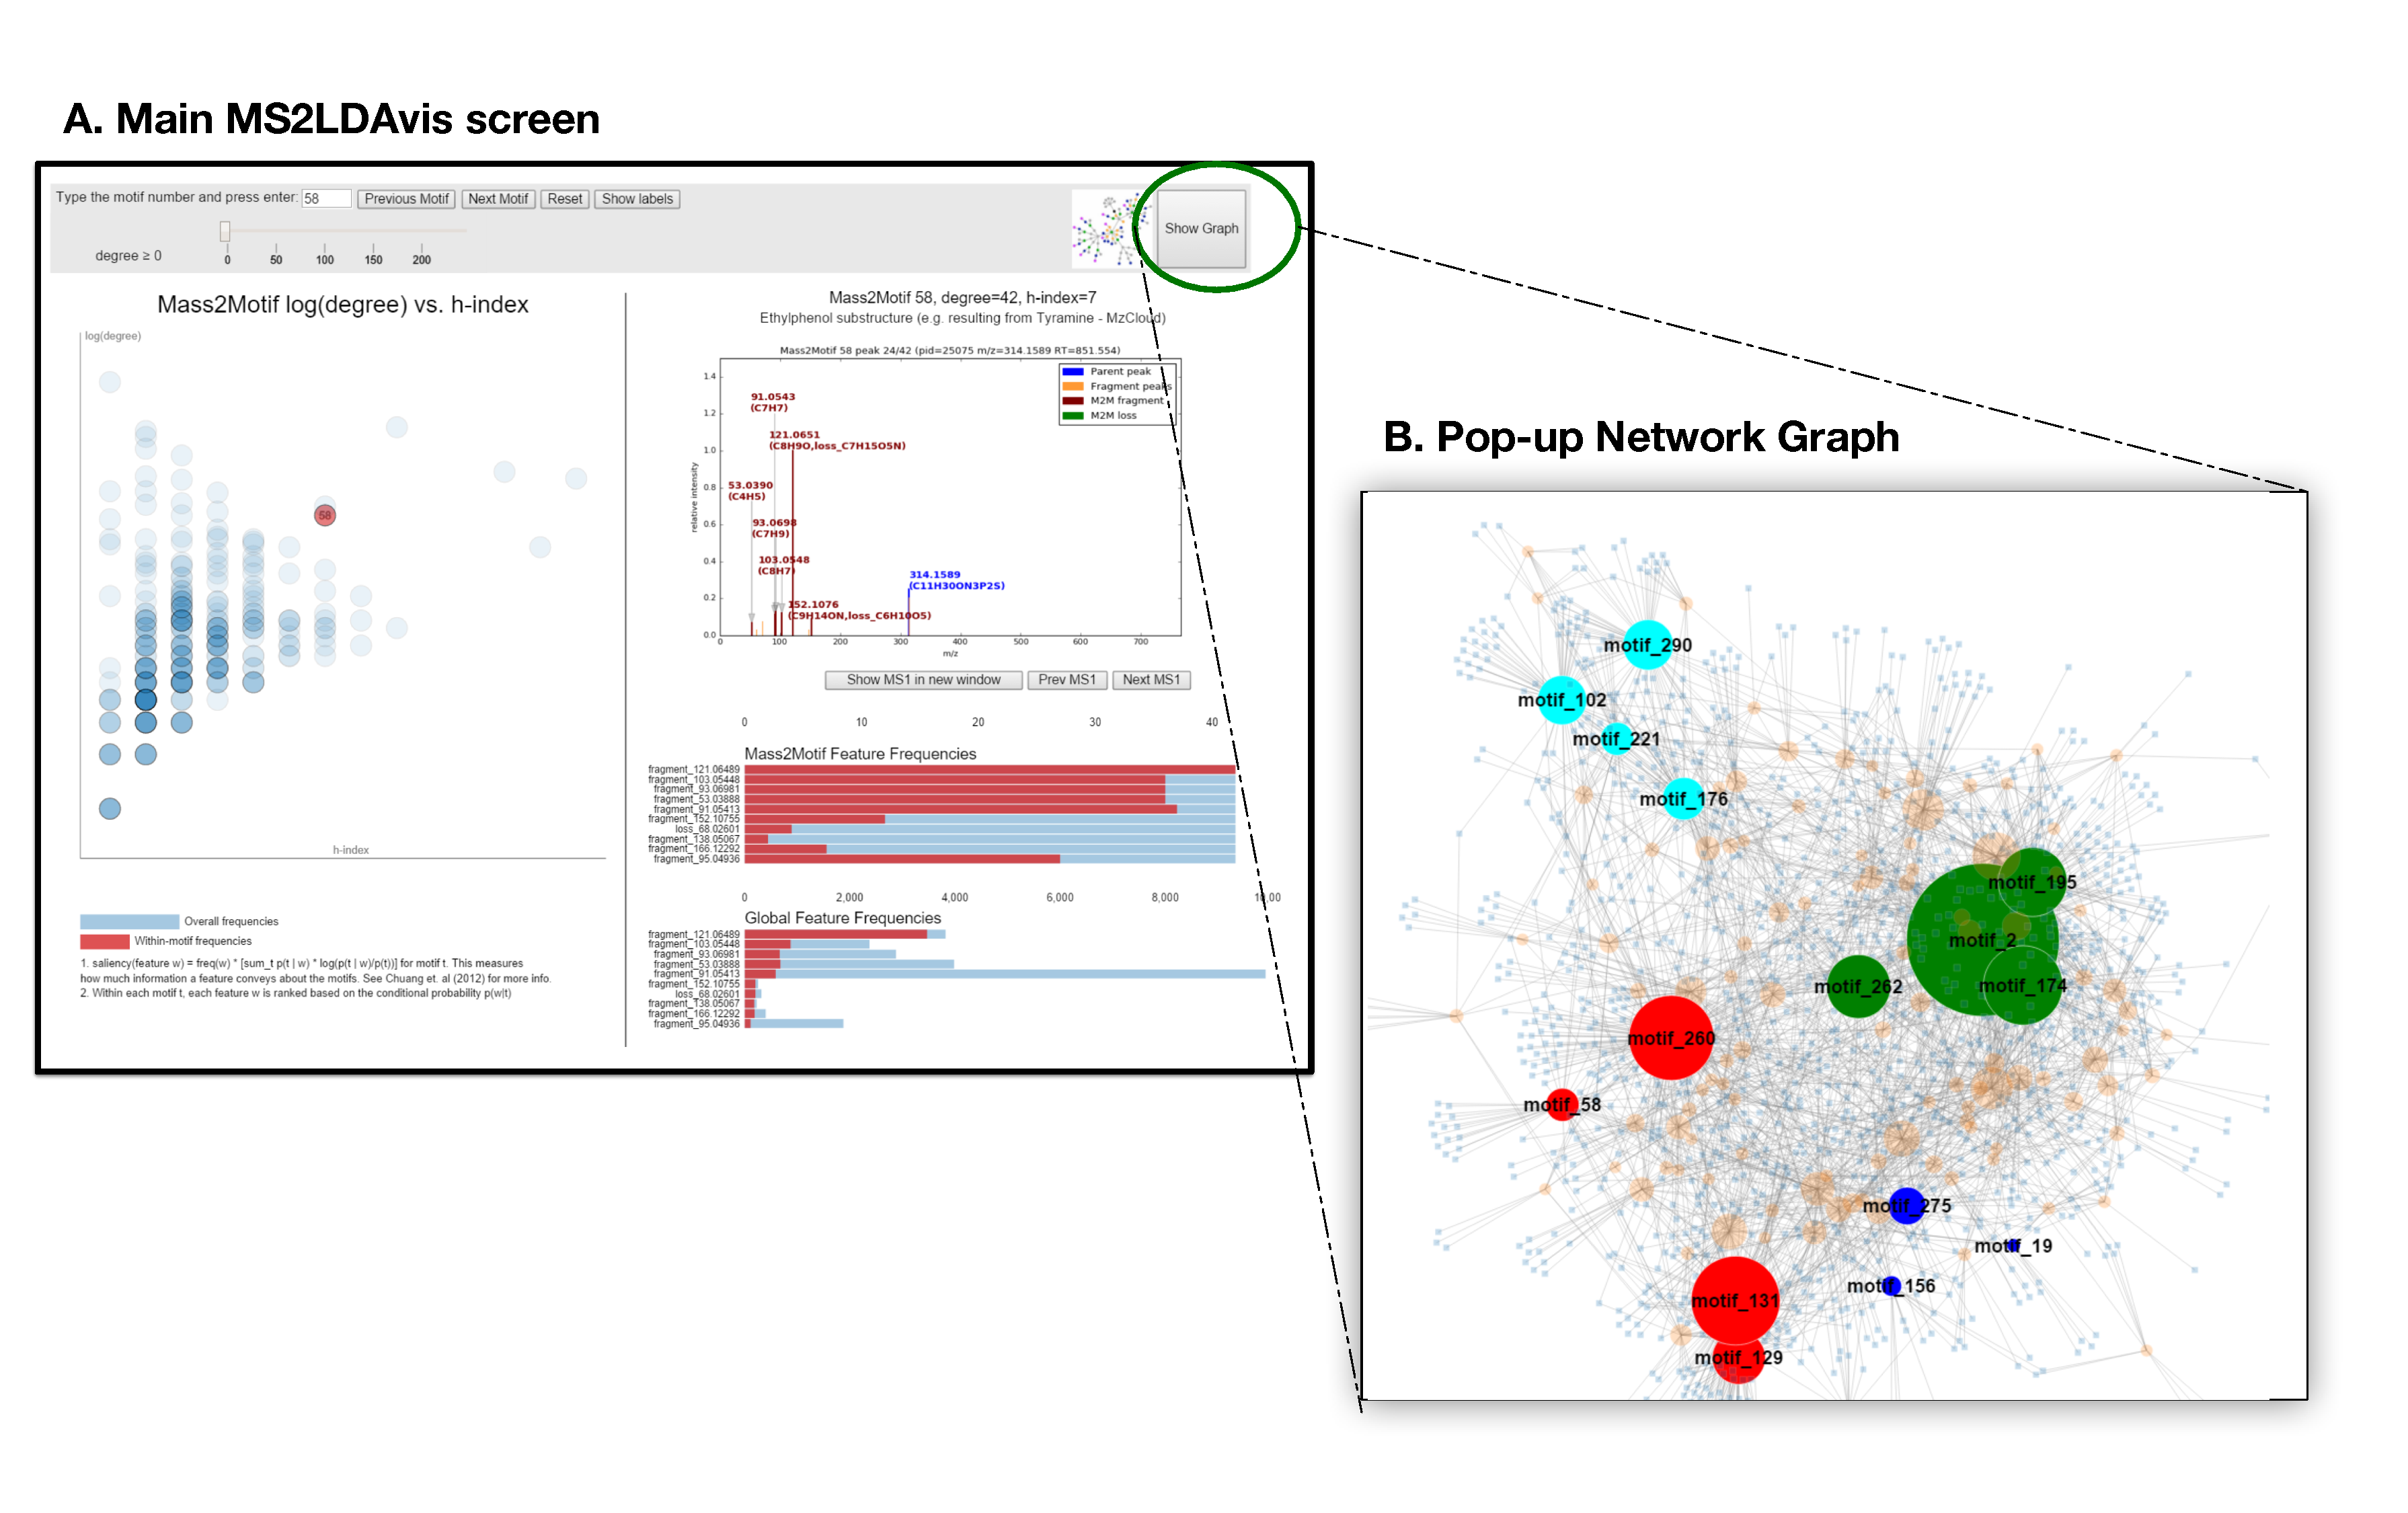
\includegraphics[width=1.0\linewidth]{07-lda/figures/figure_s3.pdf}
\centering\caption{Screenshot of MS2LDAVis. See text for explanations of the different panels.\label{fig:m2ldavis-main}}
\end{figure}

Similar to the original LDAVis, the left panel of MS2LDAVis module shows a global view of the model, whilst the right panel zooms into a specific Mass2Motif (see Figure~\ref{fig:m2ldavis-main}A). However, unlike LDAVis where topics are displayed on the left panel through multidimensional scaling that projects topics to two dimensions, the two axes in MS2LDAVis panel are the log-degree and the $h$-index of Mass2Motifs. The degree of a Mass2Motif as the number of fragmentation spectra explained by the Mass2Motif at the user-defined threshold $t_{\theta}$ on the fragmentation-spectra-to-Mass2Motif distributions ($\boldsymbol{\theta}$). The $h$-index of a Mass2Motif is defined in a similar manner to the conventional $h$-index for scientific publications of a researcher. A Mass2Motif has an index of $h$ if it has $h$ fragment or loss features obtained after setting a user-defined threshold $t_{\phi}$ on the Mass2Motif-to-features distributions ($\boldsymbol{\phi}$), each of which occur in the set of thresholded spectra at least $h$ times. Intuitively, a Mass2Motif with high degree but low $h$-index may potentially correspond to simple substructures that occur in many fragmentation spectra, while a Mass2Motif with high $h$-index but low degree are more unique and complex substructures shared by fewer MS2 spectra.

Selecting a Mass2Motif on the left panel of Figure~\ref{fig:m2ldavis-main}A changes the specific information displayed on the right panel. Fragmentation spectra that can be explained by the currently selected Mass2Motif (above the threshold $t_{\theta}$) are plotted, and clicking the ‘Previous MS1’ and ‘Next MS1’ buttons allows the flipping through consecutive spectra plots. Fragment and loss features that can be explained by the selected Mass2Motif (above the threshold $t_{\phi}$) that also occur in the plotted spectra are highlighted in bold. Two barplots can be found on the bottom right panel: the Mass2Motif Feature Frequencies displays the counts of each fragment or loss features within the entire fragmentation spectra explained by the currently selected Mass2Motif, while the Global Feature Frequencies displays the counts of the fragments or loss features within the complete data set that can be explained by the currently selected Mass2Motif.

Finally, to complement the main visualisation view, inference results can also be visualised in a pop-up network graph (Figure~\ref{fig:m2ldavis-main}B) by clicking the ‘Show Graph’ button. In the network view, Mass2Motifs and fragmentation spectra, represented by their parent MS1 peaks in the graph, form the nodes in the graph, and edges are drawn between the nodes if a spectra can be explained by a Mass2Motif above the threshold $t_{\theta}$. To minimise clutter in the graph, a slider is provided to filter nodes based on their degree values. Nodes in the graph can also be annotated and coloured according to user specifications before the visualisation interface is called. The two complementary views are linked such that clicking a Mass2Motif node on the network graph will select the corresponding Mass2Motif on the main view and vice versa. The network graph is particularly useful in exploring the relationships between Mass2Motifs and investigating which spectra can be explained by multiple Mass2Motifs.

\section{Evaluation Study}

\subsection{Evaluation Datasets\label{sub:ms2lda-datasets}}

As evaluation datasets, four beer samples representative of complex mixtures of diverse biochemically relevant compound classes (such as amino acids, nucleotides, and sugars) typical in metabolomics studies are used. The beer extracts, acquired from one home-brewed beer and three different commercially available beers, are shown in Table~\ref{tab:beer-sample-details}. One of the beer samples (Beer3) is also used for the evaluation of the alignment methods in Chapter~\ref{c:matching}. Approximately 10 ml of beer was sampled from each bottle directly after opening and stored at -20 ˚C before extractions. After thawing, i) 200 µL of beer was mixed with 600 µL of methanol/chloroform, ii) then sonicated for 5 minutes at room temperature; iii) and finally centrifuged for 5 minutes (12,000 g) at room temperature. As well as the four individual extracts, a pooled aliquot of the four beer extracts was prepared. The resulting supernatants were stored at -80 ˚C until analysis. A Thermo Scientific Ultimate 3000 RSLCnano liquid chromatography system (Thermo Scientific, CA, USA) was used. That system was coupled to a Thermo Scientific Q-Exactive Orbitrap mass spectrometer equipped with a HESI II interface (Thermo Scientific, Hemel Hempstead, UK). Thermo Xcalibur Tune software (version 2.5) was used for instrument control and data acquisition.

\begin{table}[!htbp]
\small
\centering
\begin{tabular}{|l|l|}
\hline
\textbf{Label} & \textbf{Source}                                                                                                                                                                                        \\ \hline
Beer1          & A home-brewed bottle of German Wheat Beer. \\ \hline
Beer2          & A bottle of `Jaw Glyde Ale’ brewed by JAW Brew. \\ \hline
Beer3          & A bottle of `Seven Giraffes Extraordinary Ale’ brewed by William Bros. Brewery Company. \\ \hline
Beer4          & A bottle of `Black Sheep Ale’ brewed by Black Sheep Brewery. \\ \hline
\end{tabular}
\caption{Beer samples used for evaluation dataset.}
\label{tab:beer-sample-details}
\end{table}

Following mass spectrometry, blank runs, quality control samples, and 3 standard mixes containing 150 reference compounds were run to assess the quality of the mass spectrometer and aid in metabolite annotation and identification \cite{Creek2011}. The pooled sample was run prior to and across the batch to monitor the stability and quality of the LC-MS run, whereas the samples were run in a randomized order. Immediately after acquisition, all .raw files were converted into MzXML format, thereby centroiding the mass spectra and separating positive and negative ionization mode spectra into two different mzXML files using the command line version of MSconvert (ProteoWizard). Fragmentation files were also converted into .mzML formats using the GUI version of MSconvert.  Accurate masses of standards were obtained well within 3 ppm accuracy and intensities of the quality control samples (a beer extract and a serum extract) were as expected. 

\subsection{MS2LDA Analysis}

The MS2LDA workflow was independently applied to four beer mixtures in Section~\ref{sub:ms2lda-datasets}. Our aim was to structurally characterized and annotate chemically-relevant Mass2Motifs found from the LDA analysis. A standard peak-picking metabolomics data processing workflow, based on XCMS \cite{Smith2006} and MzMatch \cite{Scheltema2011}, was used to match MS1 with MS2 spectra. On average, 1409 and 1125 sets of fragmentation spectra can be linked to MS1 peaks in positive and negative ionization mode respectively across the four datasets. These fragmentation spectra and their corresponding MS1 peaks were used as input to the MS2LDA workflow. The number of Mass2Motifs and model fit are estimated via a 4-folds cross-validation approach on one of the data file (beer3 positive ionization mode). For each test fold being held out in the data file, an estimate of the model evidence is computed after training the model on the remaining training folds in the file. A common comparison of LDA is against the multinomial mixture model (clustering). A crucial difference between LDA and standard mixture-model clustering lies in the modelling assumption that a document is a mixture of one or more topics (LDA) as opposed to each document having exactly one topic (clustering). We compare the model fit of LDA against clustering by evaluating the log evidence and perplexity on the held-out data. Perplexity measures how well a probability distribution or probability model predicts a sample and is defined as:
\begin{align*}
perplexity(W)=exp\left(\frac{\sum_{d}log(P(w_{d})}{\sum_{d}N_d}\right)
\end{align*}
where $perplexity(W)$ is the perplexity on the whole held-out test collection, $P(w_d)$ is the marginal probability of a testing spectra $d$ (integrating over all the parameters of the model), approximated via an importance sampling method \cite{wallach2009evaluation} and $N_d$ is the number of features in each testing spectra $d$. Following \cite{Griffiths2004}, we set $\alpha=K/50$ and $\beta=0.1$ during cross-validation. For mixture model clustering, a non-informative Dirichlet prior ($\alpha=K/50$, where $K$ is now the number of clusters) is set on the proportions of the mixture components and another Dirichlet prior ($\beta=0.1$) is set on cluster-specific word distributions. The Gibbs sampler for LDA and multinomial mixture model is run for 1000 samples, discarding the first 500 for burn-in. The last sample is used computing the posterior estimates. Minimal differences were found when inferred model parameters were averaged over samples in comparison to using the last sample.

\subsection{Molecular Networking Analysis}

Molecular networking analysis can be used to compare the inferred Mass2Motifs from MS2LDA against the clusters produced through cosine clustering of fragmentation spectra. For Molecular Networking analysis, the .mzXML files for the Beer fragmentation files were uploaded into the Global Natural Products Social Molecular Networking (GNPS) environment, available from http://gnps.ucsd.edu. The resulting fragmentation spectra is clustered using the MS-Cluster module with a precursor mass tolerance of 0.25 Da and a MS/MS fragment ion tolerance of 0.005 Da. Clustered fragmentation spectra originating from different files are merged to create the consensus spectra (consensus spectra containing less than 2 spectra were discarded). A graph network is created where nodes are consensus spectra and edges are drawn if the cosine similarities between nodes are above 0.55. For identification, spectra in the graph were searched against GNPS' spectral libraries, with a cosine threshold of 0.6 and having at least 4 matched fragment peaks. The resulting graph is then exported into Cytoscape and visualised using the FM3 graph layout. 

\subsection{Differential Analysis of Mass2Motifs}

By linking the MS2LDA analysis with fold changes of MS1 peaks, the differential expression of Mass2Motifs can be assessed, allowing for the identification of biochemical changes across groups of samples based on which metabolites can be explained by a Mass2Motif. The advantage of this approach is more fragmentation spectra can be explainable by the MassMotifs in comparison to the number of spectra that can be annotated or identified through conventional means of matching to spectral library. This is useful in the case of a pathway-related Mass2Motif where we can assess the change in pathway activity across groups of samples without first having to identify and map molecules to the pathway. The full-scan (MS1) LC-MS run for each Beer extract was processed using an in-house metabolomics pipeline based on XCMS \cite{Smith2006} and MzMatch \cite{Scheltema2011}. A peak table, containing information on the MS1 peak intensities, was exported to .csv files and linked to the parent ions of fragmentation spectra in MS2LDA analysis through a greedy matching scheme. The correspondence of each parent ion in MS2LDA is established by matching to its corresponding MS1 peak in the exported peak table within a specified m/z and RT tolerance values (3 ppm, 30 seconds). If there are multiple possible matches, the one with the nearest m/z difference is selected. Following this, for each Mass2Motif, a matrix is constructed where each row is a linked MS1 peak that can be explained by that Mass2Motif and the columns are intensity values from the different case and control groups used for differential analysis. This matrix is used as input to our implementation of PLAGE \cite{tomfohr2005pathway}. PLAGE is evaluated to be the best method in \cite{tarca2013comparison}, however this does not preclude using any other methods surveyed in e.g. \cite{tarca2013comparison} from being applied to the differential analysis of Mass2Motifs.

\section{Results \& Discussions}

\subsection{Model Comparison Results\label{sub:lda-model-comparison}}

To validate one of our key assumptions of Mass2Motifs represent biological building blocks (i.e. fragmentation spectrum contains more than one Mass2Motifs), we compared the LDA model at the heart of the MS2LDA workflow to a multinomial mixture model that can be used for the clustering of fragmentation spectra. The latter is equivalent to LDA with each spectrum being forced to consist of only one Mass2Motif. If MS2LDA is indeed finding structural features as conserved patterns of fragments and losses, it should explain the data with fewer Mass2Motifs than the mixture model. This is because the mixture model has to create separate Mass2Motifs for all observed combinations of structural features. Figure~\ref{fig:m2lda-perplexity} shows the perplexity for the two models on one of the Beer extracts (Beer3) as a function of K, the number of Mass2Motifs (for LDA) or clusters (for the mixture model). The lower perplexity in Figure~\ref{fig:m2lda-perplexity} demonstrates that LDA provides a better model fit on the held-out data compared to multinomial mixture model due to its lower perplexity, validating our assumption that allowing multiple conserved blocks to be present in small molecule fragmentation data is a better representation of the biochemical properties of the fragmented molecules. 

\begin{figure}[!htbp]
\centering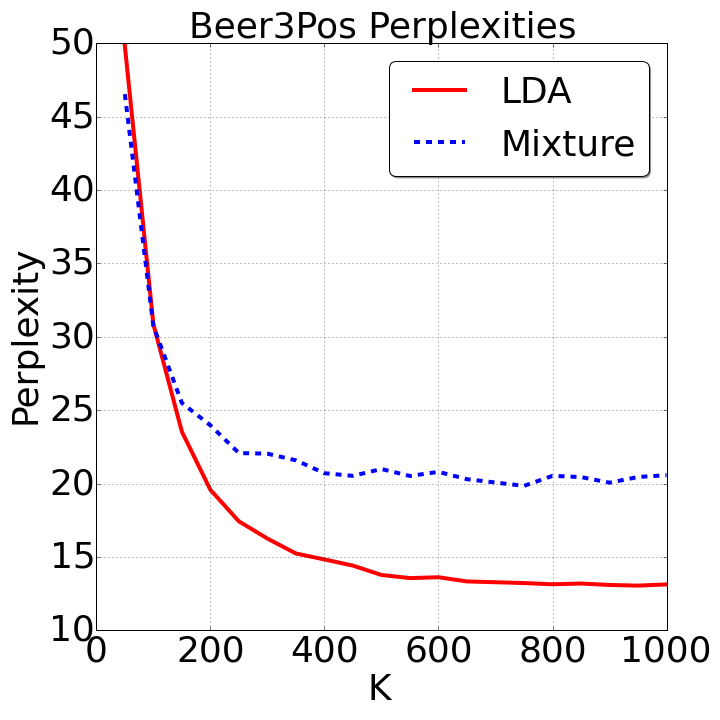
\includegraphics[width=0.5\linewidth]{07-lda/figures/perplexity.png}
\centering\caption{Results of model comparisons of LDA and multinomial mixture model on the Beer3 data. The lower perplexity values for $K>100$ demonstrates that LDA provides a better model fit on the held-out data when compared to the mixture model.\label{fig:m2lda-perplexity}}
\end{figure}

\subsection{Biological Findings\label{sub:lda-biological-findings}}

The perplexity result in Figure~\ref{fig:m2lda-perplexity} suggests the appropriate value for $K$ to be in the range of 200 to 400 at the elbow of the curve where increasing the number of topics does not result in further decrease of perplexity. With $K=300$ and other hyperparameters the same as used in cross-validation, the set of Mass2Motifs were extracted for each data file and checked for biochemical relevance. As discussed in Section~\ref{sub:ms2lda-visualisation}, the distributions over the features that make up the Mass2motifs and the distributions over Mass2motifs for each fragmentation spectrum can be thresholded for results interpretation. The default threshold values $t_{\theta}$ and $t_{\phi}$ were manually selected to be 0.05 and 0.01 respectively for visualization and data interpretation but they can easily be varied. In our analysis, Mass2Motifs with degrees ≥10 (i.e. that were present in ten or more spectra after thresholding) were manually inspected and annotated at different levels of confidence. Annotations of Mass2Motifs were established through expert knowledge and by spectral matching of the MS2 spectra containing the associated fragments and/or neutral losses to the reference spectra in MzCloud (www.mzcloud.org). Key fragment or loss features from the annotated Mass2Motifs in one sample were then searched against the list of Mass2Motifs in other samples and their correspondences established if those key fragment or loss features were present in both.

\begin{table}
\begin{centering}
\begin{tabular}{|c|c|c|c|}
\hline 
File & Total MS1 peaks & Linked to at least one structurally annotated M2M & \%\tabularnewline
\hline 
\hline 
Beer1Pos & 1282 & 951 & 74\tabularnewline
\hline 
Beer2Pos & 1567 & 1160 & 74\tabularnewline
\hline 
Beer3Pos & 1422 & 1055 & 74\tabularnewline
\hline 
Beer4Pos & 1363 & 930 & 68\tabularnewline
\hline 
\end{tabular}
\par\end{centering}
\caption{Mass2Motif coverage of MS1 peaks by percentage of MS1 peaks that can
be explained by at least one structurally annotated Mass2Motif for
the files acquired in positive ionization mode.\label{tab:ms2lda-coverage}}
\end{table}

Between 30 to 40 Mass2Motifs in each of the Beer extract could be structurally annotated as corresponding to a diverse set of biochemical substructures, including amino acid related (i.e. histidine, leucine, tryptophan, and tyrosine), nucleotide related (i.e. adenine, cytosine, and xanthine), and other molecules such as cinnamic acid, ferulic acid, ribose and N-acetylputrescine. Across the four Beer files, an average of 70\% of spectra (Table~\ref{tab:ms2lda-coverage}) include at least one annotated Mass2Motif, with Mass2Motifs related to the same substructure consistently found across multiple beers (e.g. hexose-related Mass2Motifs were present in all positive ionization mode files with degrees from 58 to more than 100). The results in Table~\ref{tab:ms2lda-coverage} demonstrates how the additional structural information from MS2LDA can aid in biological interpretation of fragmentation spectral data. Annotating just 30-40 of the discovered Mass2Motifs provides biochemical insight into 70\% of the spectra. The degree of Mass2Motifs (the number of spectra in which they occurred) varied from 1 to over 200 spectra, demonstrating the ability of MS2LDA to extract both generic and specific structural features. An example of ferulic acid (a compound present in cereals, an ingredient of beer) is given in Figure~\ref{fig:m2lda-ferulic-acid}. Three of the eleven spectra that include Mass2Motif 19 characterized as corresponding to ferulic acid substructures are shown. Conserved mass fragments, discovered in an unsupervised manner, are clearly visible across the three spectra with the most conserved highlighted in Figure ~\ref{fig:m2lda-ferulic-acid}D.   

\begin{figure}[!htbp]
\centering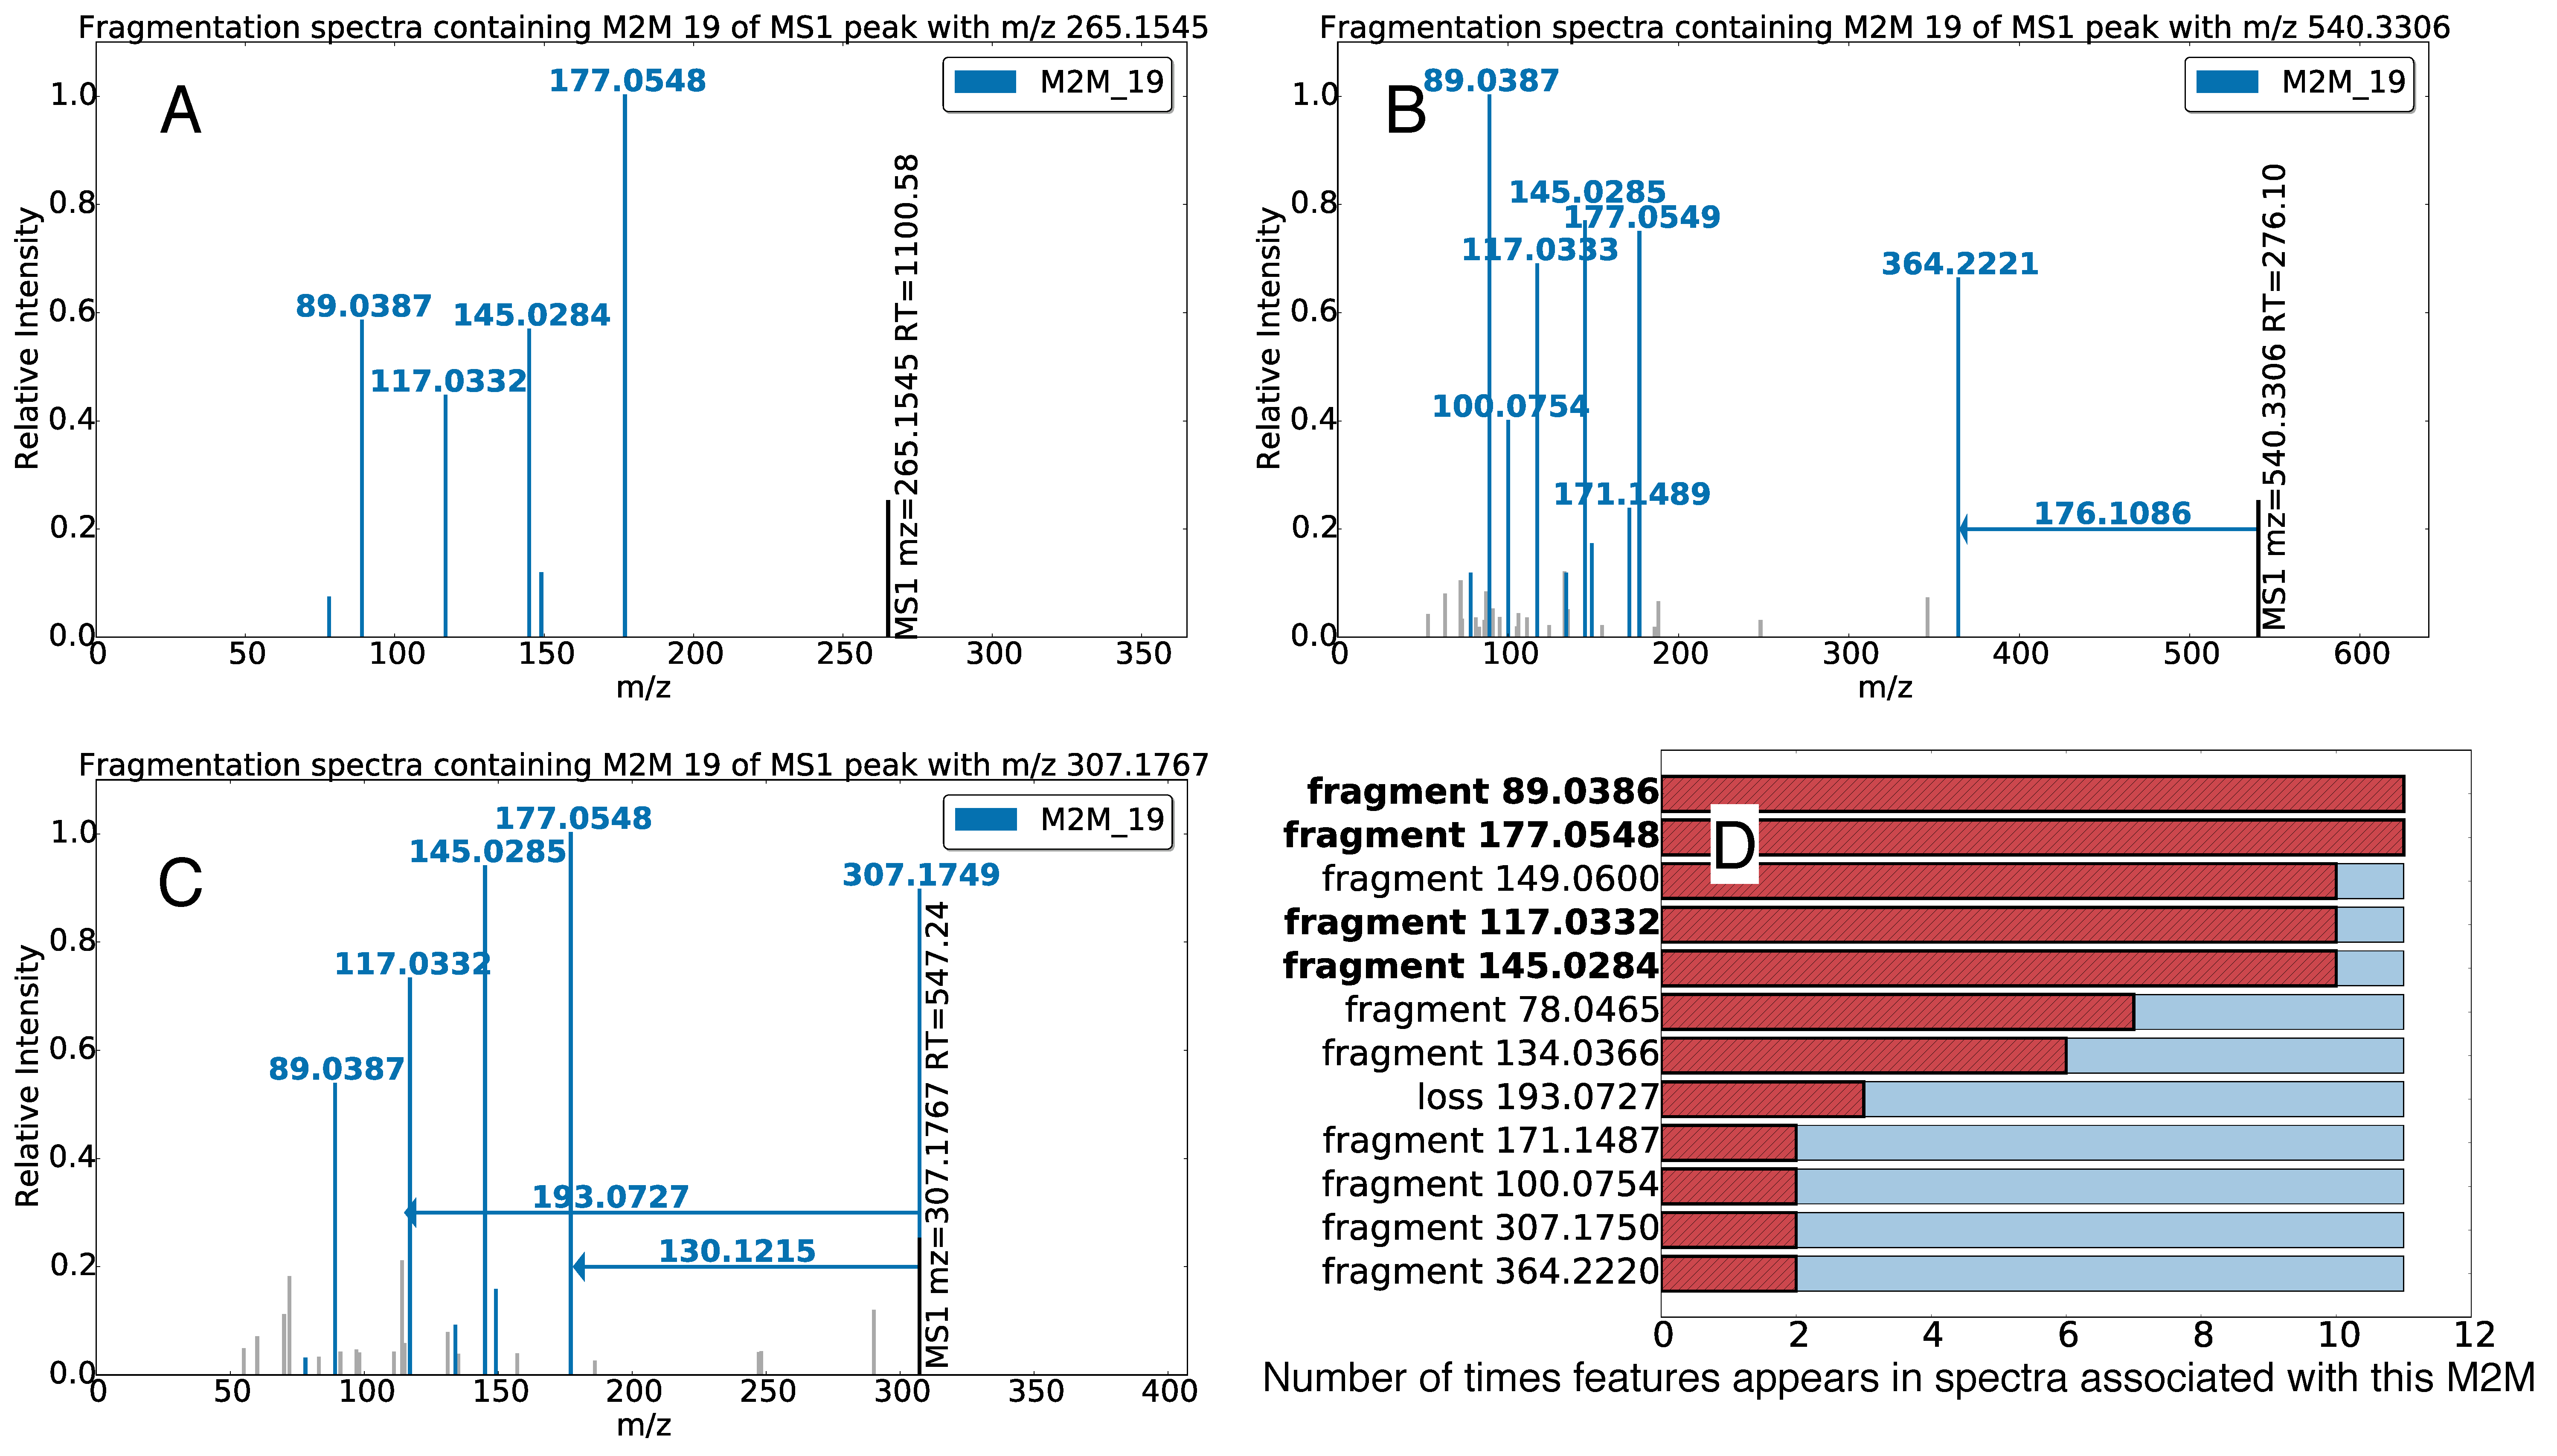
\includegraphics[width=0.8\linewidth]{07-lda/figures/ferulic_acid.pdf}
\centering\caption{Three spectra, from the beer3 positive ionization mode file, each of which includes Mass2Motif 19, annotated as the plant derived ferulic acid substructure. A-C highlight mass fragments and neutral losses (arrows originating at the precursor ions) included in Mass2Motif 19 (fragments not explained by Mass2Motif 19 are light grey). The histogram in D shows how common each fragment / loss is in the 11 instances of motif 19 found in the dataset. The abundant fragments with an m/z of 177.0545, 145.0284, 117.0332, and 89.0386 Da are most consistently present. It is of note that the neutral loss of 176.1086 and the protonated fragment of 177.0575 both relate to the complete ferulic acid substructure.\label{fig:m2lda-ferulic-acid}}
\end{figure}

A key property of the LDA model for text is that a document can be described by one or more topics. Similarly in our MS2LDA workflow, a fragmentation spectrum can now be described by one or more Mass2Motifs. Figure~\ref{fig:m2lda-combined-m2m} demonstrates this with an example of a subset of the network produced by MS2LDAvis, consisting of molecules that include two Mass2Motifs (ferulic acid and ethylphenol). All but one molecule belongs to just one of the Mass2Motifs but one belongs to both (the fragments belonging to each Mass2Motif are clearly visible). The presence of both Mass2Motifs in this molecule allows us to putatively annotate it as feruloyltyramine (314.1386 m/z; [C18H20NO4]+) despite spectral matching producing no relevant hits. For comparison, the output of spectral clustering via Molecular Networking is shown on the right of Figure~\ref{fig:m2lda-combined-m2m}. This produces clusters interpretable as ferulic acid and ethylphenol related, but as each molecule belongs to one cluster, feruloyltyramine is assigned to the ethylphenol cluster and its relationship with ferulic acid is lost. 

\begin{figure}[!htbp]
\centering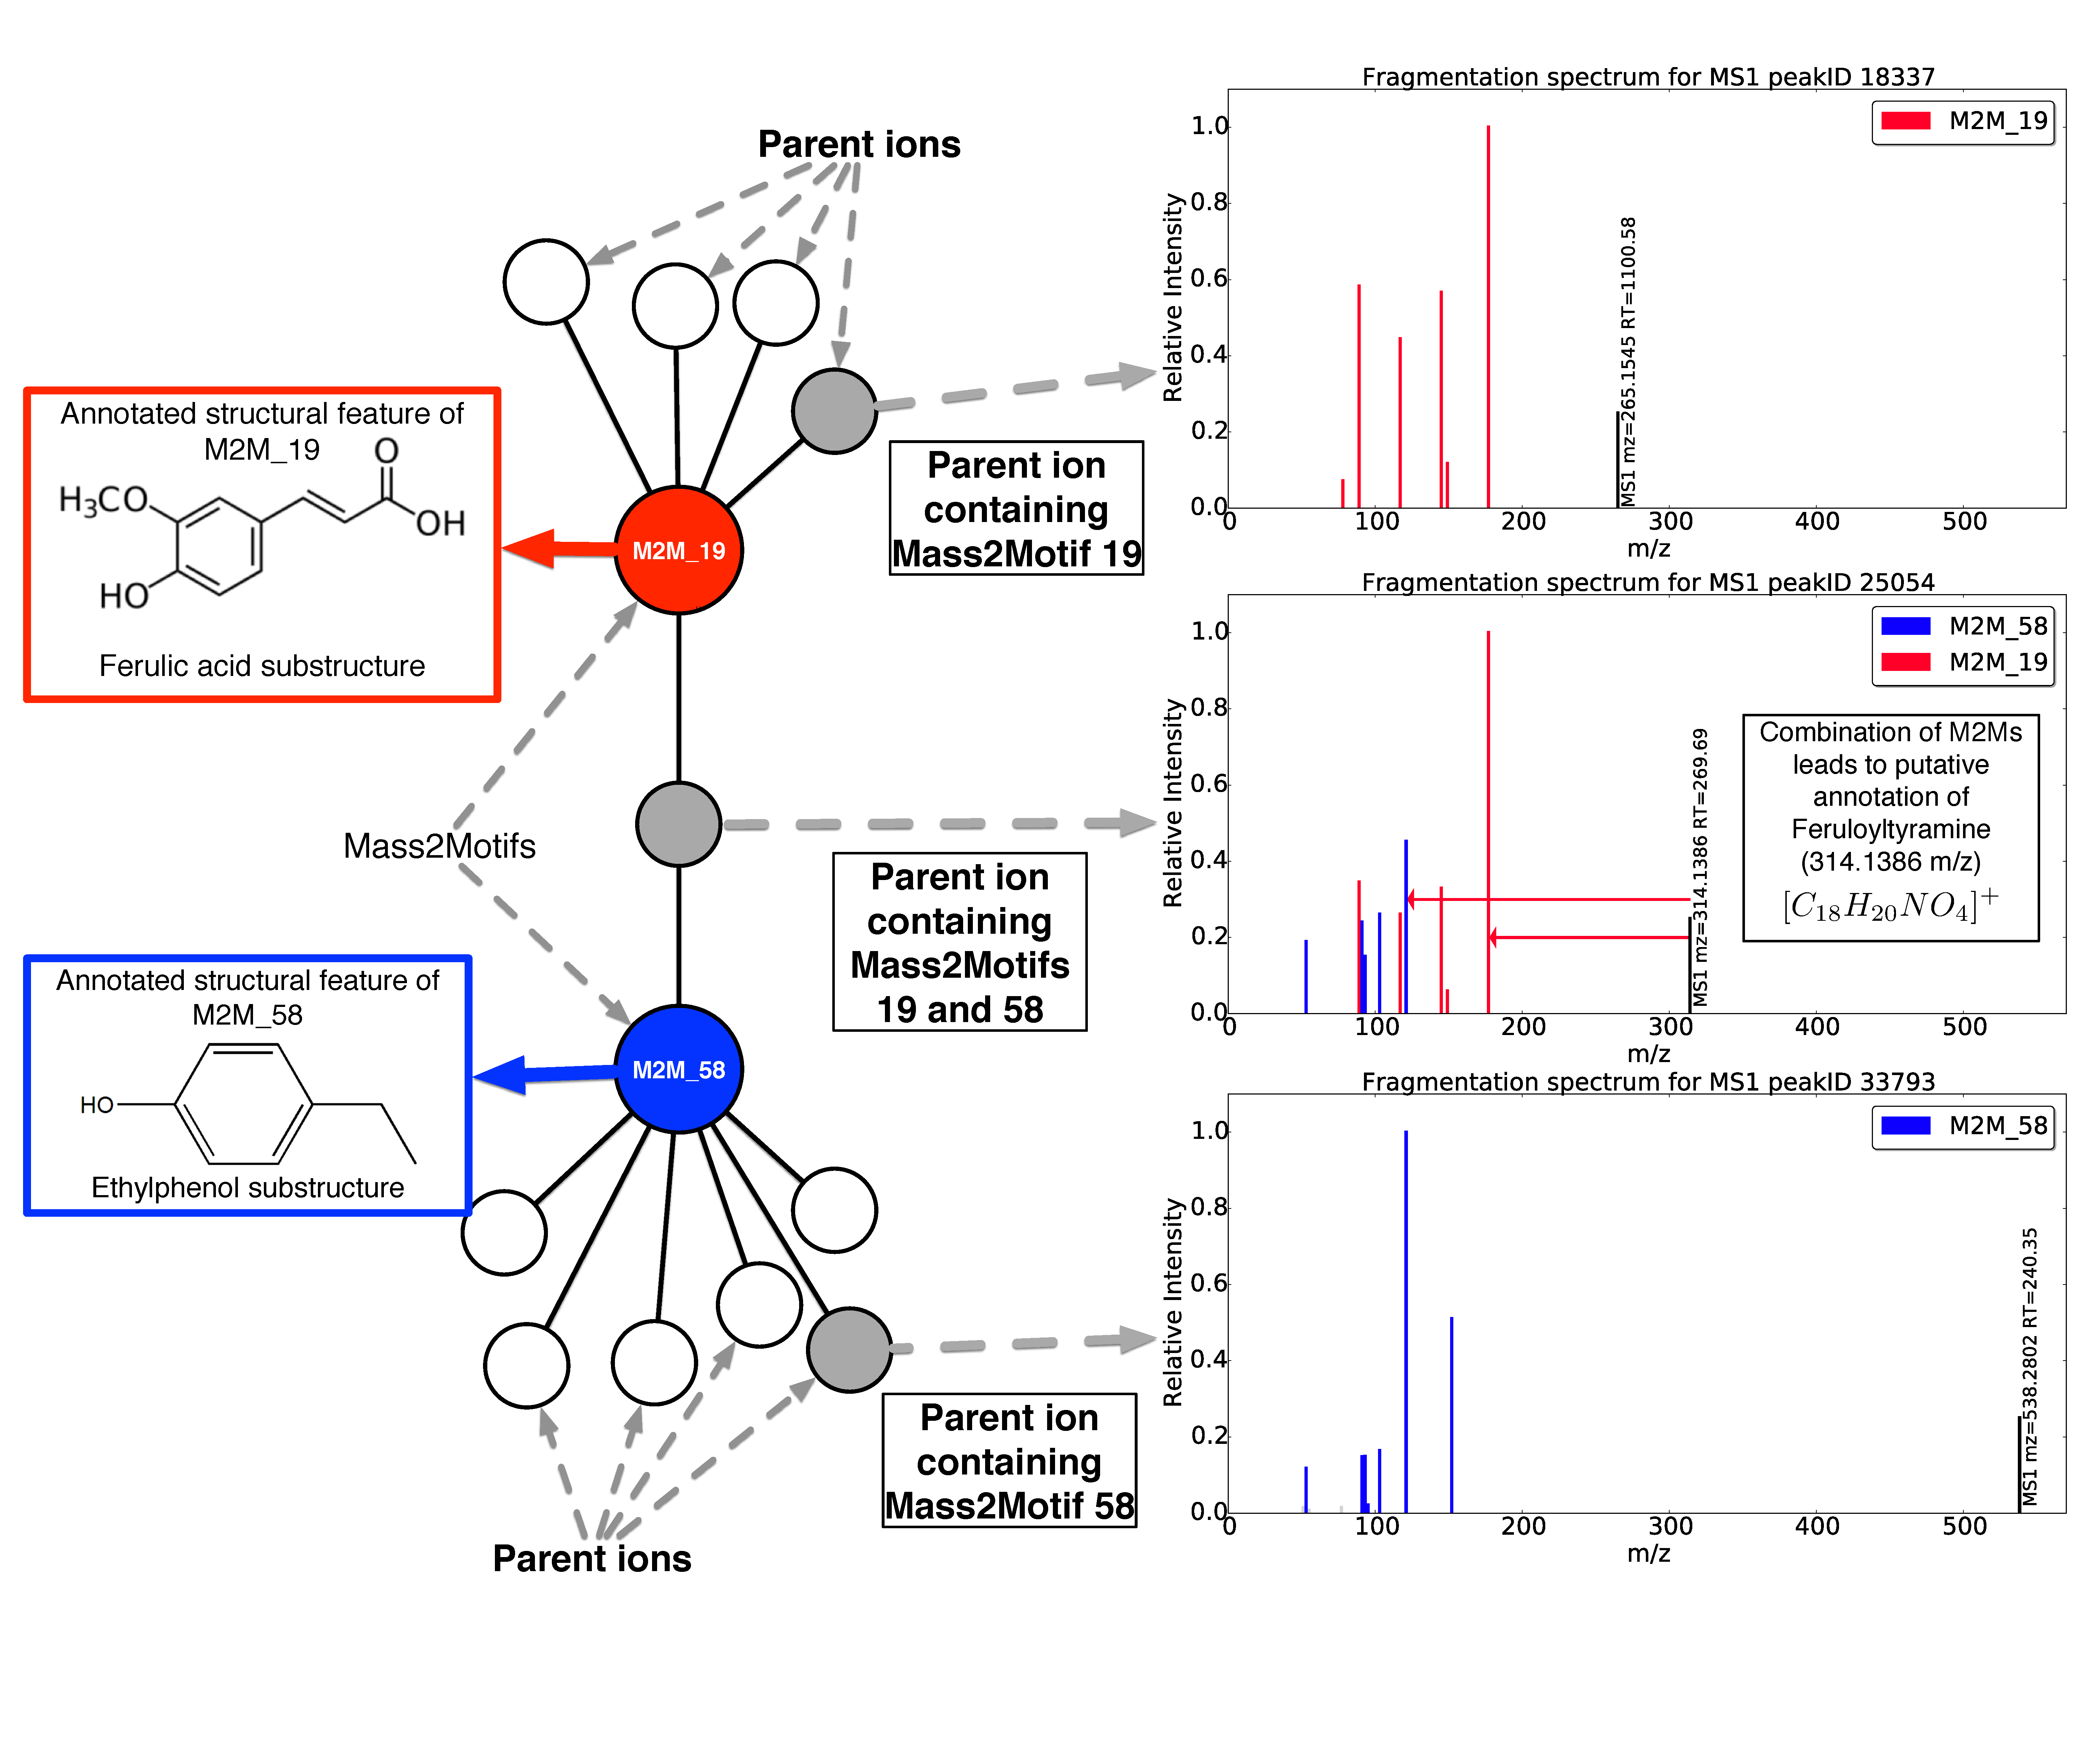
\includegraphics[width=1.0\linewidth]{07-lda/figures/combinedm2m.pdf}
\centering\caption{Mass2Motifs 19 and 58 were found to be representative of ferulic acid and ethylphenol, respectively. 11 and 42 MS1 features in the beer3 data set were explained by those two Mass2Motifs, respectively. Of those, one was explained by both Mass2Motifs, aiding in its annotation as feruloyltyramine (314.1386 m/z; [C18H20NO4]+). On the right of the plot, we show the clusters containing these three MS1 features created using the molecular networking tool (15) (top: ferulic acid, bottom: ethylphenol). The coloring of the nodes is dependent on their presence across the different beer extracts and the node size is proportional to the number of unique beer extracts the node fragmentation spectra are found in. The compound containing both Mass2Motifs is forced into the ethylphenol cluster, losing its relationship with ferulic acid.\label{fig:m2lda-combined-m2m}}
\end{figure}

Allowing each spectra to include multiple Mass2Motifs thus gives far greater potential in making de novo structural annotations of molecules, rather than each parent ion having to be assigned to a single cluster alone. This is also shown in Figure~\ref{fig:m2lda-cosine-clustering} where a matrix of cosine similarities of some parent ions drawn from the ferulic acid based cluster and the ethylphenol based cluster constructed through molecular networking is plotted. We see clear, distinct groupings of these spectra into two clusters based on the parent ions’ cosine similarities. Members of each cluster can therefore be explained by a single Mass2Motif (the ferulic acid cluster by M2M_19, and the tyramine cluster by M2M 58). However, one parent ion (the last row in Figure~\ref{fig:m2lda-cosine-clustering}) can also be explained by the two Mass2Motifs together. In cosine clustering, this parent ion would have to go into one cluster or the other based on its cosine similarity. In LDA, this spectrum can be explained by the two Mass2Motifs M2M_19 and M2M_58.

\begin{figure}[!htbp]
\centering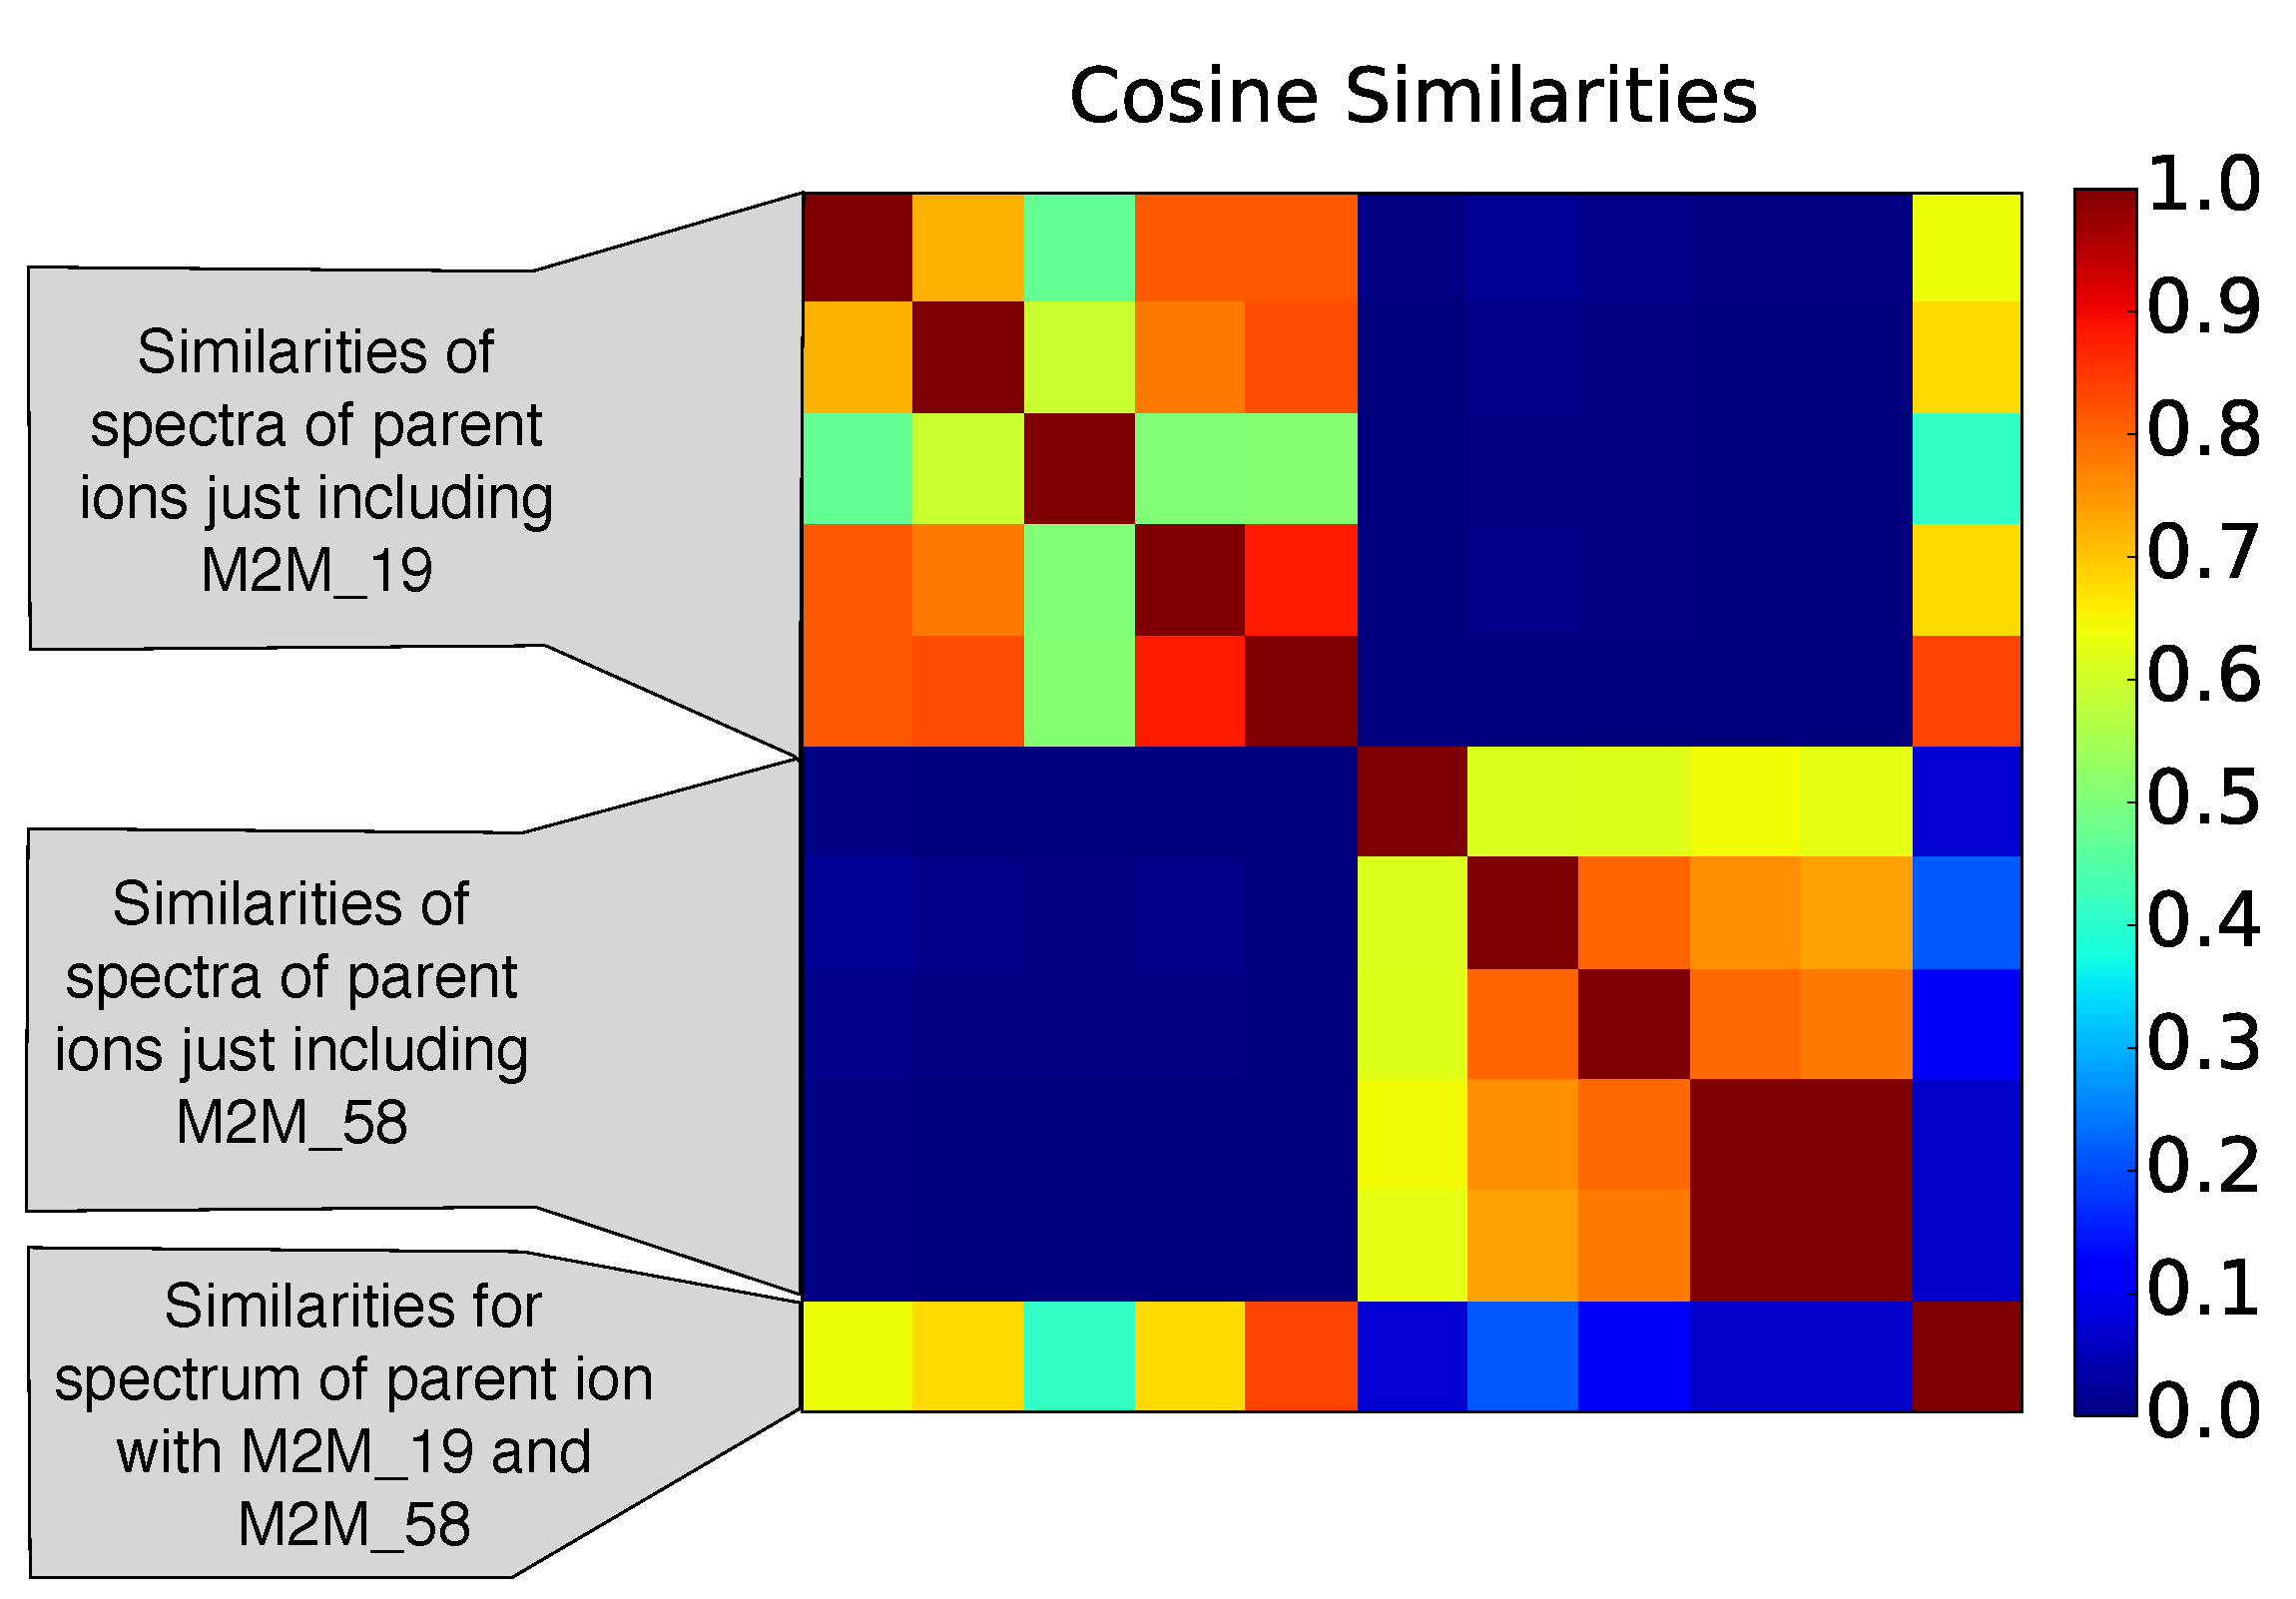
\includegraphics[width=0.6\linewidth]{07-lda/figures/figure10.pdf}
\centering\caption{Cosine clustering results of spectra drawn from the ferulic acid based cluster and the ethylphenol based cluster (similar to M2M_19 and M2M_58). The last row represents a fragmentation spectrum that contains both substructures, but in the clustering approach, the spectra will be placed into one of the clusters based on its cosine similarity. In LDA, this spectrum can be explained by Mass2Motifs that characterise both substructures.\label{fig:m2lda-cosine-clustering}}
\end{figure}

\subsubsection{Validation of Mass2Motifs Against Reference Standard Molecules}

Reference standard molecules present in the beer extracts can be identified based on chromatographic co-elution and exact mass. As the identities of the parent MS1 peaks produced by the standard molecules is known, we can validate our structurally annotated Mass2Motifs. Of the 45 standard molecules we could identify, 38 included one or more annotated Mass2Motif --- despite the fact that the original Mass2Motifs annotation was made independently of reference molecule characterisation --- with 32 containing Mass2Motifs that correspond to known biochemical features consistent with the structural features of the standard molecules. Figure~\ref{fig:m2lda-standards} shows examples with fragmentation spectra colored by Mass2Motif. The spectra for phenylalanine (Figure~\ref{fig:m2lda-standards}A) and histidine (Figure~\ref{fig:m2lda-standards}B) share Mass2Motif 262, indicating the presence of a free (underivatized) carboxylic acid group. The loss of CHOOH (Mass2Motif 262) is in fact a common characteristic for many other underivatized amino acids and free organic acids and was associated with 10 of the 18 amino acids structures matched from the standards (the remaining 8 prefer alternative fragmentation routes – e.g. see the amine loss in tryptophan, Figure 3C). The other Mass2Motifs (115, 241) in Figures~\ref{fig:m2lda-standards}A and~\ref{fig:m2lda-standards}B are related to phenylalanine and histidine, respectively. Finally, Figure~\ref{fig:m2lda-standards}D is the MS2 spectrum of adenosine, which consists of an adenine molecule conjugated to a ribose sugar molecule. The two associated Mass2Motifs (156, 220) represent these two biochemically relevant structural features (i.e., adenine substructure and a loss corresponding to a ribose sugar).  

% Spectra can include multiple Mass2Motifs. In each of Figures~\ref{fig:m2lda-standards}A to~\ref{fig:m2lda-standards}D, we observe two or more Mass2Motifs. We know of no other method that can do this without training spectra consisting of known structures, or a priori knowledge of interesting feature combinations. Multiple Mass2Motifs can also explain the same feature in one spectrum, i.e. the fragments 110.0717 (C5H8N3, [M+H]+)  and 120.0803 (C8H10N, [M+H]+) in Figures~\ref{fig:m2lda-standards}A and \ref{fig:m2lda-standards}B are explained by Mass2Motifs 241 and 115 and also by the 46.0054 loss (CHOOH) of Mass2Motif 262. This demonstrates the manner in which MS2LDA decomposes molecules into their constituent building blocks, allowing for de novo metabolite annotation (see Section~\ref{sub:ms2lda-identification}). 

\begin{figure}[!htbp]
\centering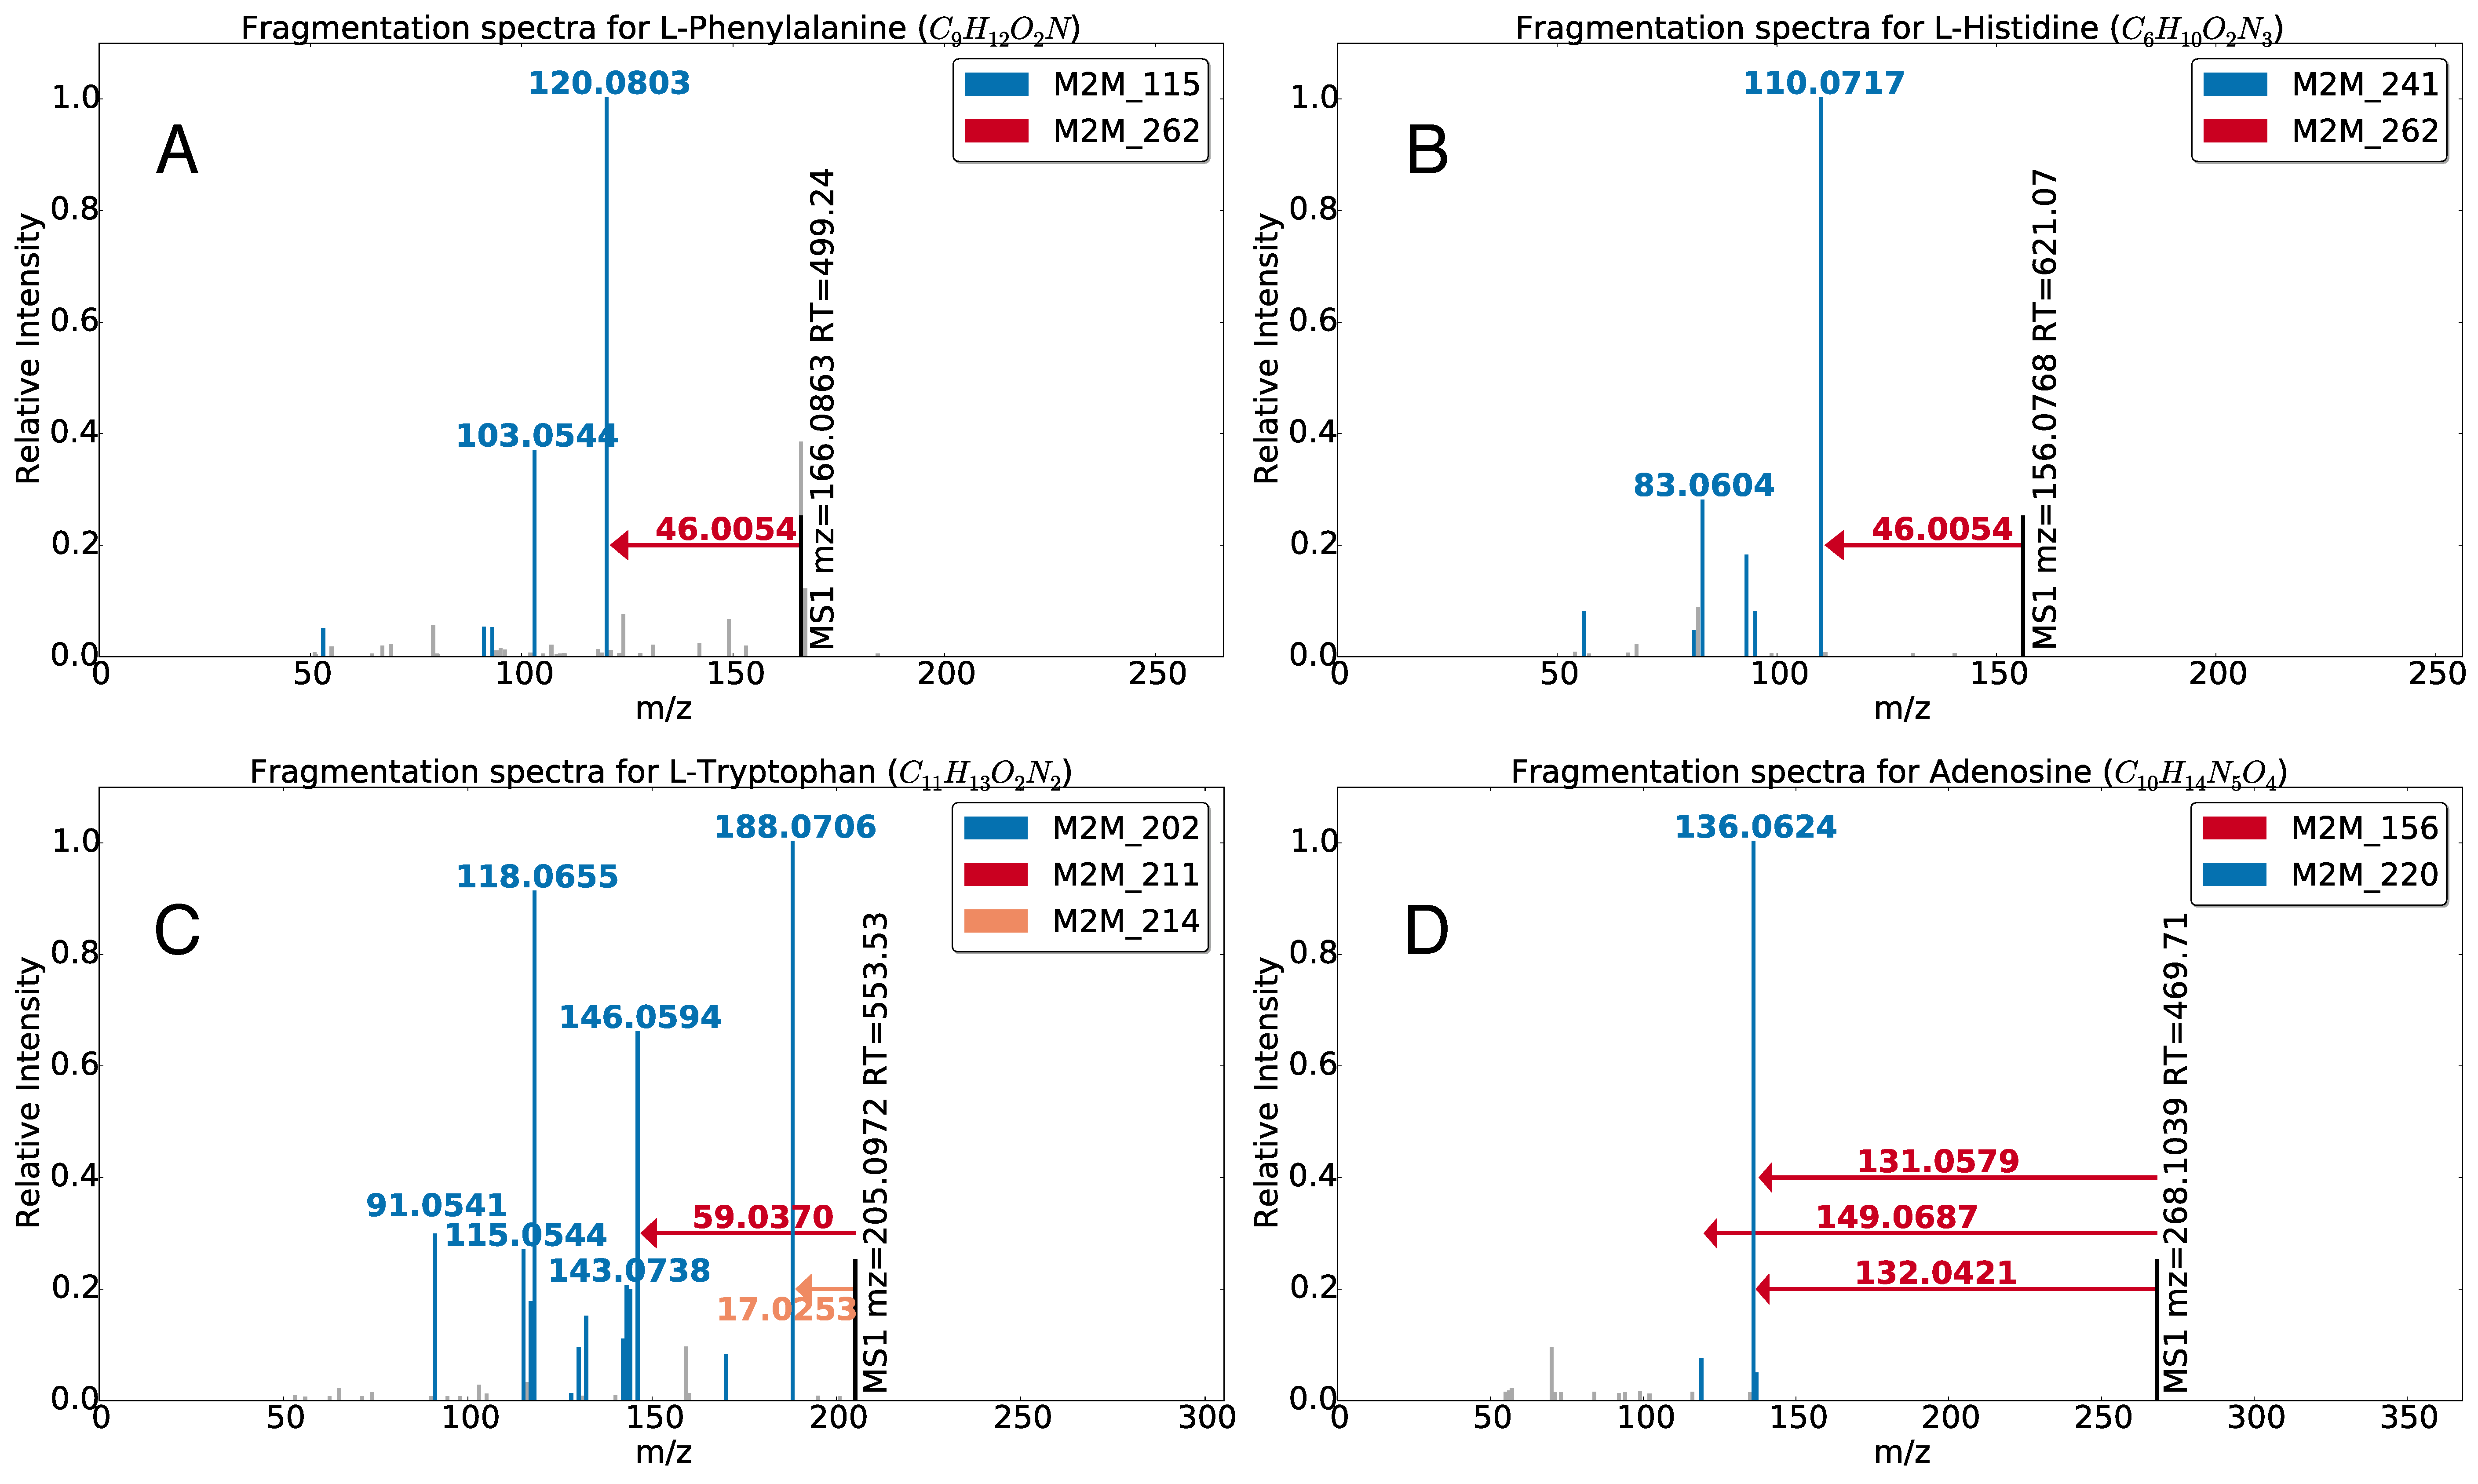
\includegraphics[width=0.8\linewidth]{07-lda/figures/standards.pdf}
\centering\caption{Mass2Motif spectra of identified standard molecules A) L-histidine, B) L-phenylalanine, C) L-tryptophan, and D) adenosine. Characterized motifs (see Table~\ref{tab:ms2lda-standards}) are indicated by color.\label{fig:m2lda-standards}}
\end{figure}

% Preview source code for paragraph 1

\begin{table}
\small
\begin{centering}
\begin{tabular}{| c | p{4cm} | c | p{3.5cm} | p{2.5cm} |}
\hline 
Mass2Motif & Annotation & Degree & Fragment or Loss Features & Elemental Formula\tabularnewline
\hline 
\hline 
115 & {[}phenylalanine-CHOOH{]}-based substructure.  & 28 & fragment\_120.0808, fragment\_103.0546, fragment\_91.0541 & C8H10N, \newline C8H7, \newline C7H7\tabularnewline
\hline 
156 & {[}ribose (pentose, C5-sugar)-H2O{]}-related loss.  & 22 & loss\_132.0421 & C5H8O4 \tabularnewline
\hline 
202 & {[}tryptophan-NH3{]}-related substructure.  & 15 & fragment\_118.0654, 
fragment\_117.0571, 
fragment\_91.0541, 
fragment\_130.0645,
fragment\_188.0706 & C8H8N, \newline
C8H7N, \newline
C7H7, \newline
C9H8N, \newline
C11H10NO2\tabularnewline
\hline 
211 & N-acetylputrescine substructure.  & 24 & loss\_59.0370, \newline
fragment\_114.0912, 
fragment\_72.0447, 
fragment\_60.0448 & C2H5NO, 
C6H12NO, C3H6NO, 
C2H6NO\tabularnewline
\hline 
214 & amine loss.  & 57 & loss\_17.0247  & NH3\tabularnewline
\hline 
220 & adenine substructure.  & 32 & fragment\_136.0629, 
fragment\_119.0351 & C5H6N5, 
C5H3N4\tabularnewline
\hline 
241 & histidine substructure.  & 21 & fragment\_110.0718, 
fragment\_156.0769, 
fragment\_93.0450, 
fragment\_95.0608 & C5H8N3, 
C6H10N3O2, 
C5H5N2, 
C5H7N2\tabularnewline
\hline 
262 & combined loss of H2O and CO \textendash{} indicative for free carboxylic
acid group (COOH).  & 90 & loss\_46.0053  & CH2O2 \tabularnewline
\hline 
\end{tabular}
\par\end{centering}
\caption{Annotations of the Mass2Motifs associated to the fragmentation spectra
of the peaks generated by the standard molecules shown in Figure~\ref{fig:m2lda-standards}. The degree of
a Mass2Motif indicates the number of MS2 fragmentation spectra in
the beer3 positive ionization mode data having fragment or loss features
that can be explained by the Mass2Motif (at the specified thresholding
level). \label{tab:ms2lda-standards}}
\end{table}
 
\subsubsection{Differential Analysis of Mass2Motifs}

Being able to annotate more metabolites is beneficial when investigating the changes in metabolite intensity across multiple samples. As MS2LDA groups metabolites in a biochemically relevant manner, we can go a step further and consider the differential expression of Mass2Motifs in a manner similar to approaches taken in transcriptomics where it is common to consider the shared differential expression (DE) of a group of related transcripts as indicative of their contribution to a common aspect of cellular biology \cite{tarca2013comparison}. Using PLAGE \cite{tomfohr2005pathway}, we assessed the DE of each Mass2Motif based on the intensity changes of the relevant MS1 peaks between beers 2 and 3. Figure~\ref{fig:m2lda-heatmaps} shows MS1 intensities of metabolites explained by two Mass2Motifs with high PLAGE scores (note that for a high PLAGE score changes in expression do not need to be in the same direction). As an example of the kind of biochemical insight this provides, in Beer3, the free guanine (Figure~\ref{fig:m2lda-heatmaps}A) is more abundant whereas in Beer2, guanine-conjugates are more abundant. Similarly, the molecules associated to the pentose Mass2Motif (Figure~\ref{fig:m2lda-heatmaps}B) show DE between the extracts. It is the grouping performed by MS2LDA that exposes such insights from fragmentation data. We investigated whether or not similar outcomes can be achieved with with spectral similarity clustering. With this approach, the 12 pentose-related metabolites were distributed across 10 clusters rather than appearing in a single grouping, hiding the potentially relevant correlated intensity change. Comparing against spectral similarity clustering, the molecules explainable by the pentose Mass2Motif (Figure~\ref{fig:m2lda-heatmaps}B) are distributed over 10 spectral clusters. The results suggest how MS2LDA analysis can be used to pull together the sets of fragment and loss features for differential analysis that would otherwise have not been found through spectral similarity clustering alone.

\begin{figure}[!htbp]
\centering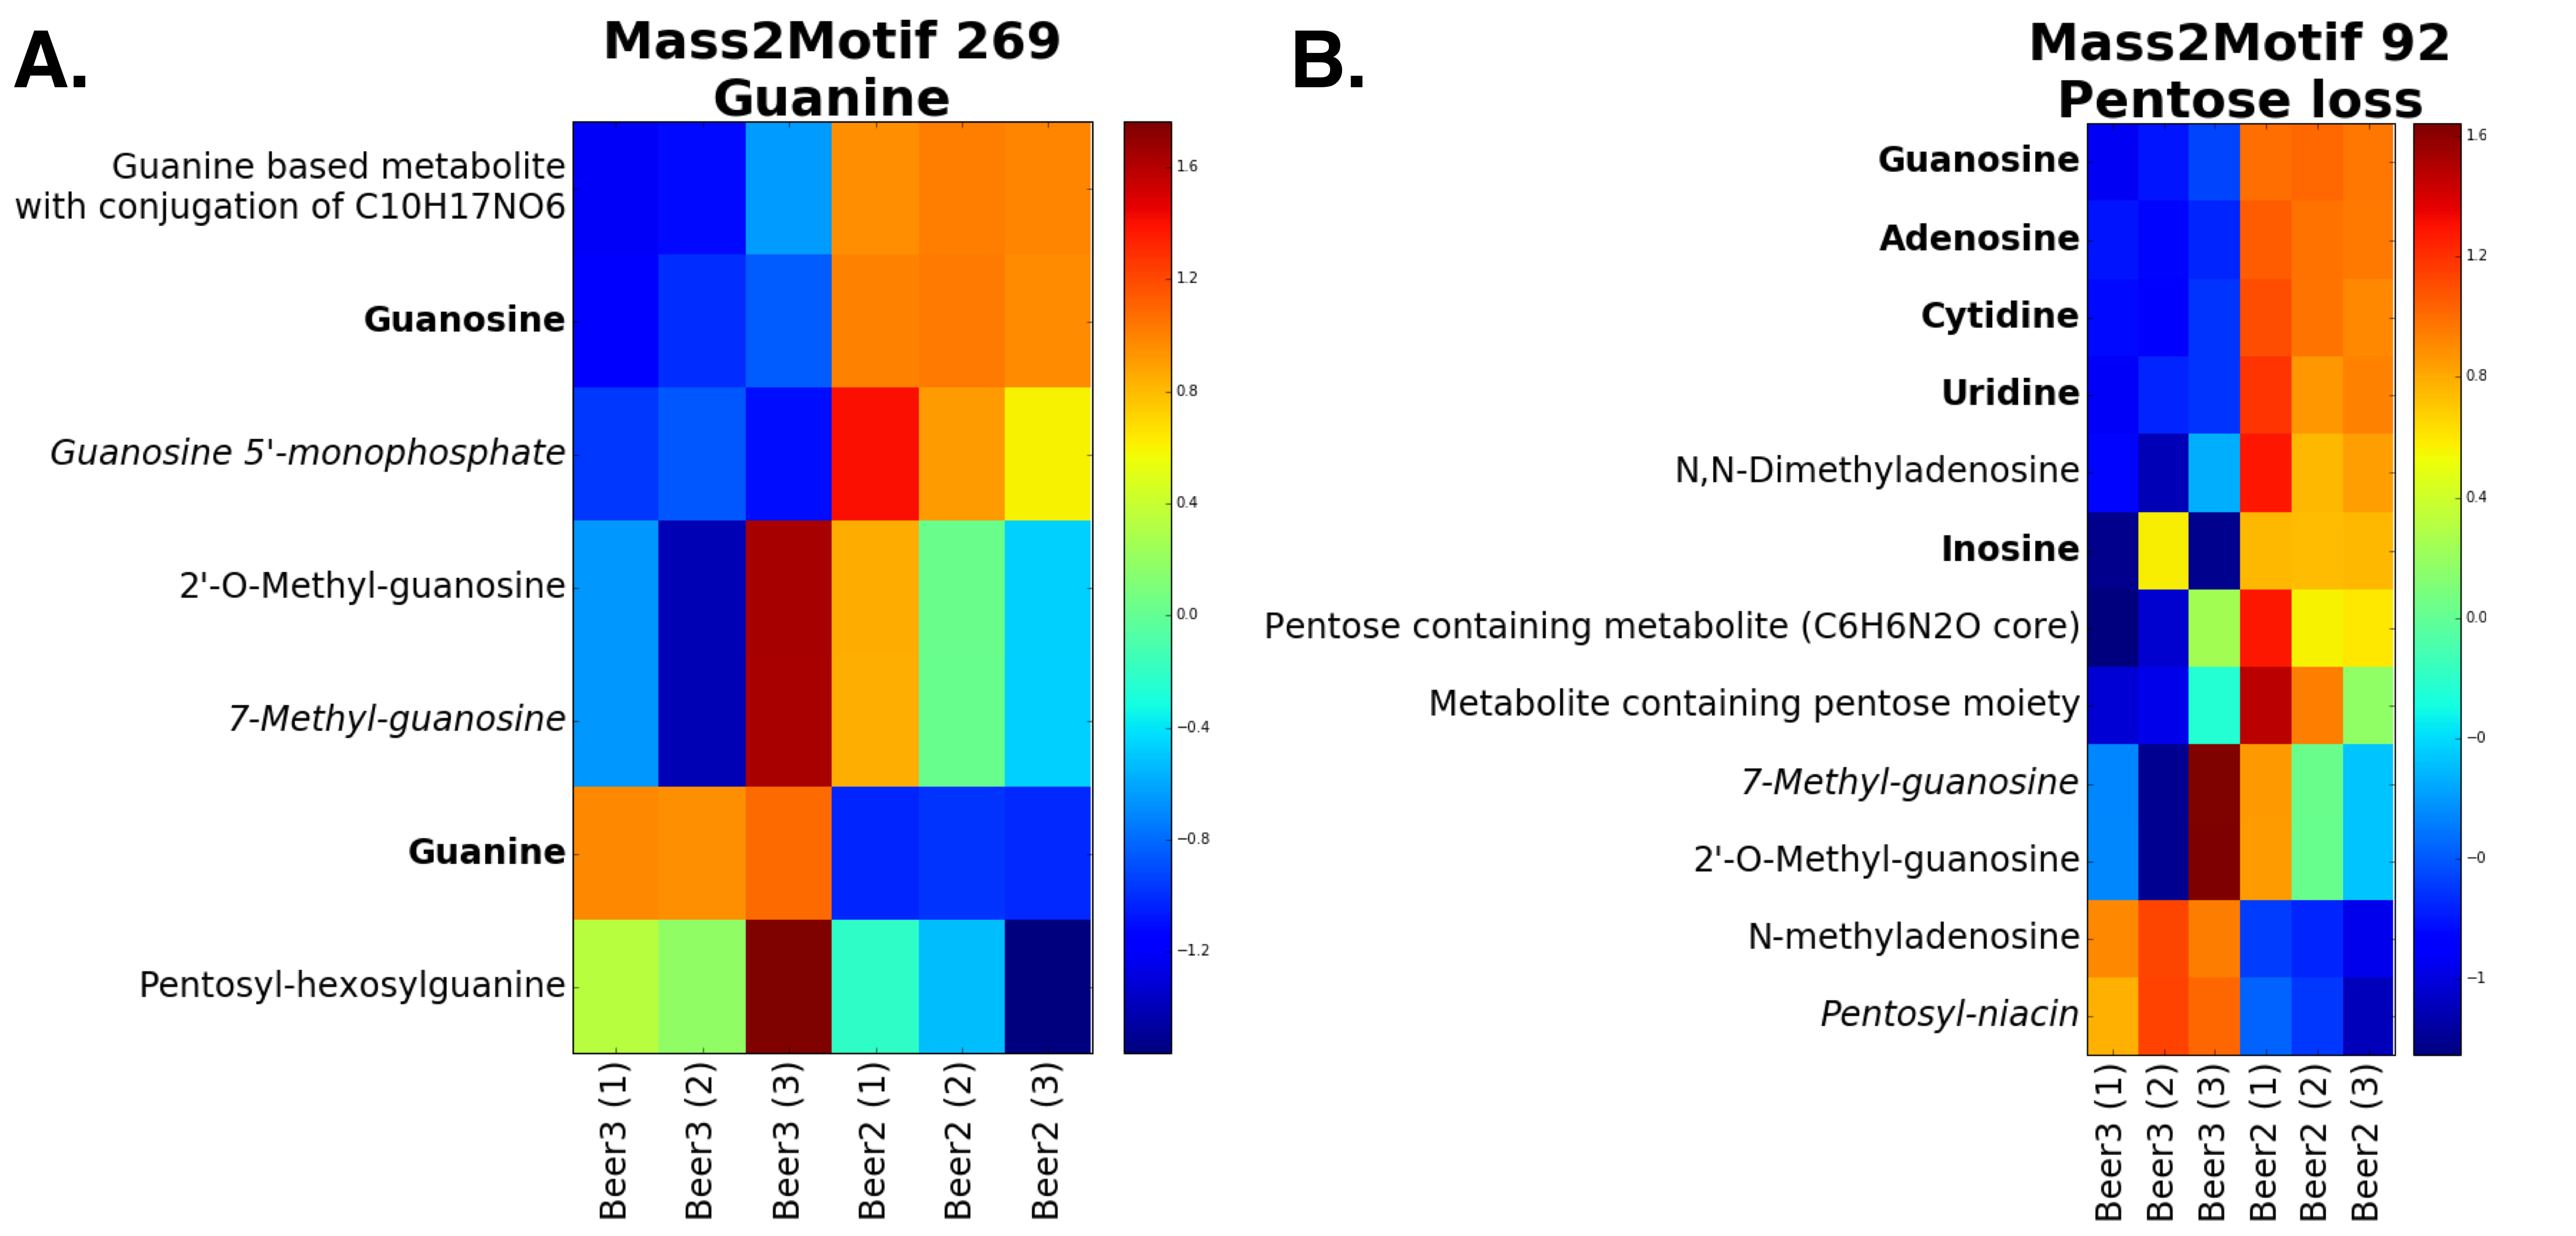
\includegraphics[width=1.0\linewidth]{07-lda/figures/heatmaps.png}
\centering\caption{Log fold change heat-maps for the A) guanine and B) pentose loss Mass2Motifs. Each row is an annotated parent MS1 peak and columns represent different beer extracts. Bold names for parent MS1 peaks could confidently be matched to reference compounds. \label{fig:m2lda-heatmaps}}
\end{figure}

\section{Substructure Discoveries Across Many Fragmentation Files}

Manual inspection of the results revealed that many Mass2Motifs, related to the same substructures, are consistently present in two or more beers. This is despite each sample being processed independently through MS2LDA. For example, the hexose-related Mass2Motifs are present in all positive ionization mode beer files with degrees from 58 to more than 100 in each beer. The results suggest that we can jointly model the presence or absence of Mass2Motifs across many input files at once, eliminating the necessary but tedious matching of Mass2Motifs across files if they were to be inferred independently for each input file.

\subsection{Multi-file LDA Model}

Metabolomics dataset consist of fragmentation spectra in multiple input files, where each file is generated from measurements of a technical or biological replicate. In this manner, Mass2Motif distributions over fragment and loss features are shared across files, but within each file, fragmentation spectra have their own file-specific probabilities of observing certain Mass2Motifs. When only a single input file is provided, the multi-file LDA model reduces to the standard LDA model. 

In the proposed multi-file LDA model, the observation on the $n$-th fragment or loss feature in the $d$-th fragmentation spectra in file $f$ ($w_{dn}^f$) is conditioned on the assignment of feature $w_{dn}^f$ to some $k$-th global Mass2Motif multinomial distribution that is shared across files. This assignment is denoted by the indicator variable $\boldsymbol{z}_{dn}^f$, so $\boldsymbol{z}_{dn}^f=k$ if feature $n$ from fragmentation spectra $d$ in file $f$ is assigned to the $k$-th Mass2Motif. The probability of seeing certain Mass2Motifs for each $d$-th fragmentation spectra in file $f$ is then drawn from a multinomial distribution with a parameter vector $\boldsymbol{\theta}_{d}^f$. This parameter vector $\boldsymbol{\theta}_{d}^f$ is in turn drawn from a prior Dirichlet distribution having a symmetric parameter $\alpha^f$. 
\begin{align}
\boldsymbol{z}_{dn}^f \vert \boldsymbol{\theta}_{d}^f &\sim Multinomial(\boldsymbol{\theta}_{d}^f) \label{eq:dir-multi-1a}\\
\boldsymbol{\theta}_{d}^f \vert \alpha &\sim Dirichlet(\alpha^f) \label{eq:dir-multi-1b}
\end{align}
As in the case of standard LDA, the $k$-th multinomial distribution for a Mass2Motif is characterised by the parameter vector $\boldsymbol{\phi}_{\boldsymbol{z}_{dn}^f}$, with $\boldsymbol{\phi}_{\boldsymbol{z}_{dn}^f}$ drawn from a prior Dirichlet distribution, here having a symmetric parameter $\beta$. 
\begin{align}
\boldsymbol{w}_{dn}^f \vert \boldsymbol{\phi}_{\boldsymbol{z}_{dn}^f} &\sim Multinomial(\boldsymbol{\phi}_{\boldsymbol{z}_{dn}^f}) \label{eq:dir-multi-2a} \\
\boldsymbol{\phi}_{k} \vert \beta &\sim Dirichlet(\beta) \label{eq:dir-multi-2b}
\end{align}

Inference in the multi-file LDA model is again performed via a collapsed Gibbs sampling scheme. The conditional probability of $P(\boldsymbol{z}_{dn}^f=k \vert \boldsymbol{w}_{dn}^f, ...)$ of the assignment of feature $n$ in spectra $d$ file $f$ to Mass2Motif $k$ is given by eq. (\ref{eq:multifile-lda-gibbs}).
\begin{equation}
P(\boldsymbol{z}_{dn}^f=k \vert \boldsymbol{w}_{dn}^f, ...) \propto P(\boldsymbol{w}_{dn}^f \vert \boldsymbol{z}_{dn}^f=k, ...) P(\boldsymbol{z}_{dn}^f=k \vert ...)
\label{eq:multifile-lda-gibbs}
\end{equation}
where $...$ denotes any other parameters being conditioned upon but not explicitly listed. Similar to the derivation of standard LDA, we can marginalise over all $\boldsymbol{\phi}_k$ parameters in the likelihood term, $P(\boldsymbol{w}_{dn}^f \vert \boldsymbol{z}_{dn}^f=k, ...)$ of eq. (\ref{eq:multifile-lda-gibbs}), to obtain:
\begin{equation}
P(\boldsymbol{w}_{dn}^f \vert \boldsymbol{z}_{dn}^f=k, ...) \propto \frac{\sum_{f} c_{kn}^f + \beta}{\sum_{n}\sum_{f} c_{kn}^f + N\beta}
\label{eq:multifile-lda-gibbs-likelihood}
\end{equation}
where $\sum_{f} c_{kn}^f$ is the total number of features from all files that are currently assigned to Mass2Motif $k$, excluding the current feature being sampled in the current iteration of Gibbs sampler, and $N$ the total number of features obtained from binning across all files. For the prior term $P(\boldsymbol{z}_{dn}^f=k \vert ...)$, marginalising over all $\boldsymbol{\theta}_{d}^f$ parameters produces as in the standard LDA:
\begin{equation}
P(\boldsymbol{z}_{dn}^f=k \vert ...) \propto  c_{dk}^f + \alpha
\label{eq:multifile-lda-gibbs-prior}
\end{equation}
with $c_{dk}^f$ the number of features from document $n$ in file $f$ currently assigned to Mass2Motif $k$, excluding the current feature being sampled. 
Putting the prior and likelihood terms together, the following predictive distribution is obtained for the assignment of feature $n$ from document $d$ file $f$ to Mass2Motif $k$:
\begin{equation}
P(\boldsymbol{z}_{dn}^f=k \vert \boldsymbol{w}_{dn}^f, ...) \propto (c_{dk}^f + \alpha) \cdot \frac{\sum_{f} c_{kn}^f + \beta}{\sum_{n}\sum_{f} c_{kn}^f + N\beta}
\label{eq:multifile-lda-gibbs-combined}
\end{equation}

In each iteration of the Gibbs sampling, the information on the current feature $n$ in spectra $d$ file $f$ being sampled is removed. Reassignment of the feature to a Mass2Motif is performed by sampling $\boldsymbol{z}_{dn}^f$ from the distribution specified by eq. (\ref{eq:multifile-lda-gibbs-combined}). Finally, for each Gibbs sample, the spectra-to-Mass2Motif distributions, the $\boldsymbol{\theta}_{d}^f$ for each spectra, and the Mass2Motif-to-feature distributions, $\boldsymbol{\phi}_k$ for each Mass2Motif, are obtained using the expectation of the Dirichlet-Multinomial distributions defined in eqs. (\ref{eq:dir-multi-1a})-(\ref{eq:dir-multi-1b}) for the spectra-to-Mass2Motif distributions and also the Mass2Motif-to-feature distributions in eqs. (\ref{eq:dir-multi-2a})-(\ref{eq:dir-multi-2b}). For each $\boldsymbol{\theta}_{d}^f$ and $\boldsymbol{\phi}_k$ given the state of the Markov chain in a sample, we obtain:
\begin{align}
E[\boldsymbol{\theta}_{d,k}^f] &= \frac{c_{dk}^f+\alpha}{c_{d}^f+K\alpha} \\
E[\boldsymbol{\phi}_{k,n}] &= \frac{c_{kn}+\beta}{c_{k}+N\beta}
\end{align}
where $c_{dk}^f$ is the number of features from spectra $d$ in file $f$ assigned to Mass2Motif $k$, $c_{d}^f$ is the number of all features in file $f$ assigned to Mass2Motif $k$, $c_{kn}$ is the number of feature $n$ from all files that are assigned to Mass2Motif $k$ and $c_k$ is the number of all features assigned to Mass2Motif $k$. Using either the last sample or the entire set of posterior samples after burn-in averaged at a certain thinning interval to ensure low auto-correlation between subsequent samples, estimates on $\boldsymbol{\theta}_{d}^f$ and $\boldsymbol{\phi}_k$ can be obtained.

\subsection{Results \& Discussion}

On the dataset of four Beer extracts in positive ionisation mode processed through multi-file LDA using the same hyperparameters as the individual LDA. For data interpretation, initially, the same threshold values on $t_{\theta}$ and $t_{\phi}$ were selected as the previous single-file analysis (0.05 and 0.01 respectively). Table~\ref{tab:multifile-results} shows the results of five global Mass2Motifs that could be matched to the individual LDA results in Section~\ref{sub:lda-biological-findings}. The results in Table~\ref{tab:multifile-results} shows that multi-file LDA produces comparable results on the Mass2Motifs composition. This is entirely expected given that the four Beer extracts used for evaluation share similar metabolic profiles and correspondingly, have many substructures in common. 

\begin{table}[!tbhp]
\small
\centering
\begin{tabular}{|l|l|p{3.8cm}|}
\hline
Mass2Motif & Annotation                & Top Features Above Threshold                                                                                                                                                                           \\ \hline
M2M\_17           & Ferulic acid substructure & \textbf{fragment\_177.05478}, \textbf{fragment\_89.03865}, \textbf{fragment\_145.02844}, \textbf{fragment\_117.03319}, loss\_58.98941, \newline fragment\_163.03887, \textbf{fragment\_149.05998}, loss\_88.09967 \\ \hline
M2M\_155          & Histidine substructure    & \textbf{fragment\_110.07161}, \textbf{fragment\_156.07687}, fragment\_83.06041, \textbf{fragment\_93.04511}, fragment\_82.05246, fragment\_209.10558, \textbf{fragment\_95.06057}, loss\_167.08663, fragment\_81.04494, loss\_191.0615 \\ \hline
M2M\_115          & Leucine substructure      & \textbf{fragment\_86.09653}, \textbf{fragment\_132.10165}, fragment\_69.07013, fragment\_332.112, fragment\_143.11763 \\ \hline
M2M\_95           & Water loss substructure   & \textbf{loss\_18.01031}, \newline fragment\_314.0859, \newline fragment\_296.07259                                                                                                              \\ \hline
M2M\_232          & Asparagine substructure   & \textbf{fragment\_136.06231}, loss\_162.03459, \textbf{fragment\_119.0354}, loss\_162.00534, \newline fragment\_137.04623 \\ \hline
\end{tabular}
\caption{Five global Mass2Motifs inferred from multi-file LDA. For each Mass2Motif, the top features above threshold are listed. Features characterised as key to the substructure from the previous individual LDA analyses are shown in bold.}
\label{tab:multifile-results}
\end{table}

Information from all files contribute to the inference of global Mass2Motifs, and the fact that global Mass2Motifs consistent with our previous characterisation in Section~\ref{sub:lda-biological-findings} still emerge suggests the same underlying patterns of fragment and loss features to be present in each Beer extract. Figure~\ref{fig:multifile-lda} shows four example fragmentation spectra originating from different Beer extracts --- jointly inferred by multi-file LDA as containing the Mass2Motif characterised to be the ferulic acid substructure. While this can be achieved from independently running LDA on each file, the tedious matching of common Mass2Motifs that occur across files can now be eliminated. Inspections on the degree (the number of spectra associated to a Mass2Motif above the user-defined threshold $t_{\theta}$) of the five Mass2Motifs in Table~\ref{tab:multifile-results} revealed that with minor adjustment of $t_{\theta}$, the same sets of fragmentation spectra previously associated to the listed Mass2Motifs can all be recovered. 

\begin{figure}[!htbp]
\centering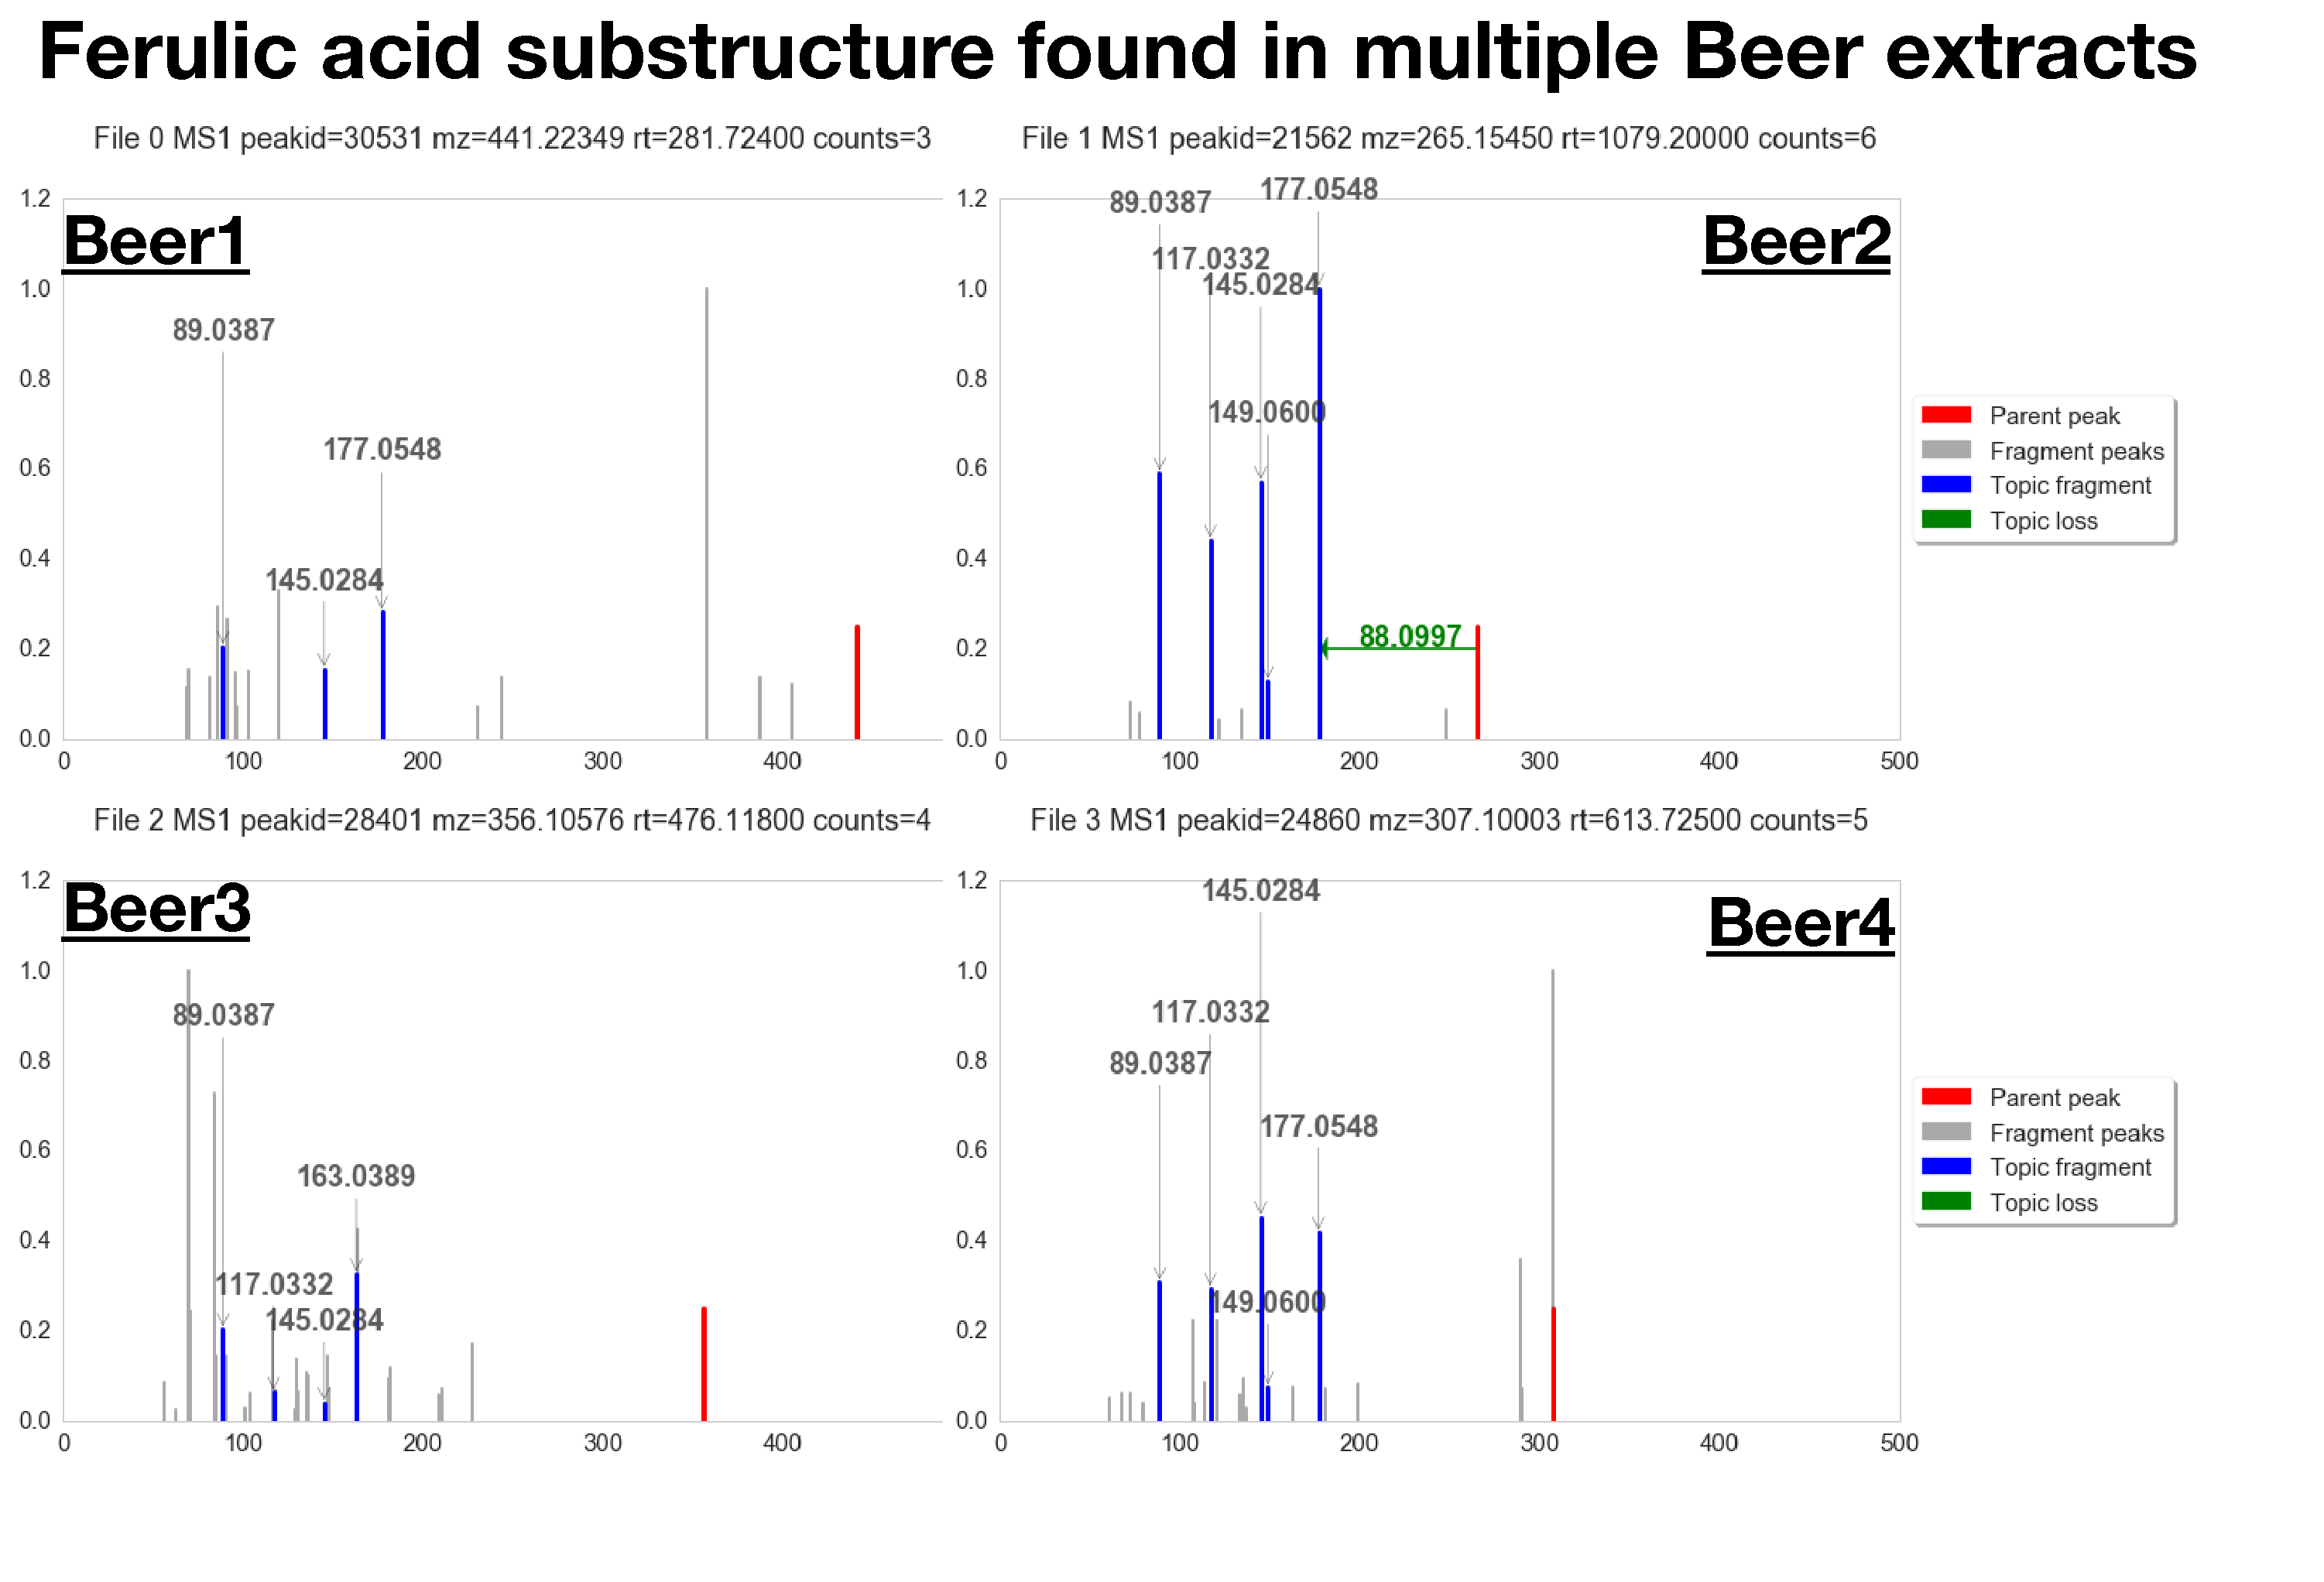
\includegraphics[width=1.0\linewidth]{07-lda/figures/multifile.pdf}
\centering\caption{Fragmentation spectra from different Beer extracts found by multi-file LDA to contain the same Mass2Motif (M2M_17) characterised as the ferulic acid substructure.\label{fig:multifile-lda}}
\end{figure}

\section{Conclusion}

We have introduced MS2LDA, a pipeline that simplifies fragmentation data by exploiting the parallels between MS fragmentation data and text documents. The pipeline performs all steps required in the analysis: the preparation of a co-occurrence matrix of fragment and loss features in fragmentation spectra, the LDA analysis, and the graphical visualization of the resulting output. Evaluation of the workflow on beer extracts result in numerous informative patterns of concurrent mass fragmental and neutral loss, termed Mass2Motifs, which we could annotate as biochemically-relevant substructures. The MS2LDA approach is markedly different from other advanced spectral analysis tools as multiple Mass2Motifs can be associated with one metabolite, and determination of the key mass fragments or neutral losses that are part of a conserved structural motif is unsupervised. 

As future work, we envision developing a larger library of characterised Mass2Motifs from data sets produced on a diverse range of analytical platforms and different sample types. An extension of the standard LDA model, in form of the multi-file LDA model, is proposed to handle Mass2Motif inference from multiple data sets, and conditioned on having an efficient implementation, such a model can be used in large-scale clinical and metabolomic studies. The prior information on which candidate Mass2Motifs an MS2 spectrum might include could also be incorporated into the MS2LDA workflow, resulting in a semi-supervised model. Other LDA-based techniques developed for text (e.g. hierarchical LDA \ref{griffiths2004hierarchical}) are also likely to offer benefits in this domain. We anticipate that MS2LDA to be particularly useful in research areas such as clinical metabolomics, pharmacometabolomics, environmental analysis, natural products research and nutritional metabolomics, as it can quickly and in an unsupervised manner recognize substructure patterns related to drugs, pollutants, and food-derived molecules, respectively. Furthermore, when linked with fold changes from MS1 data, allows the researcher to focus on clusters of metabolites that share expression changes and a chemical substructure.